\section{The random coefficients logit model}\label{sec:08-model}

The random coefficients logit model describes a population of consumers who differ in how much they value
each product characteristic and how much they dislike paying. Each consumer makes a logit choice given her
tastes. Market shares average these individual choice probabilities over the distribution of tastes in the
population. This section builds the model in steps. We start from the general random utility formulation of
\citet{BerryLevinsohnPakes1995} and specialize it to the linear form used in most applications
\citep{Nevo2000a,Nevo2001}. We then discuss income effects, normalizations and the maintained assumptions. The
section ends with the market share function, special cases, the role of the unobserved product characteristic,
and the data the model requires.

\subsection{Primitives}\label{sec:08-primitives}

We observe markets $t = 1, \dots, T$. A \emph{market} is a population of consumers who face the same set of
products at the same prices. Its definition depends on the data. \citet{BerryLevinsohnPakes1995} treat the
national new car market in each year from 1971 to 1990 as a market, so $T = 20$. \citet{Nevo2001} observes
ready-to-eat cereal sales in a panel of cities and defines a market as a city-quarter, which gives 1,124
markets \citep[p.~517]{Nevo2000a}. Other studies split one geographic market into income groups
\citep[p.~517]{Nevo2000a}.

Market $t$ offers the inside products $j \in \mathcal{J}_t = \{1, \dots, J_t\}$ and an outside good $j = 0$,
which stands for not buying any of the inside products. The market has $M_t$ potential consumers, its
\emph{market size}. If $q_{jt}$ units of product $j$ are sold, its market share is
$s_{jt} = \frac{q_{jt}}{M_t}$, and the outside share is $s_{0t} = 1 - \sum_{j \in \mathcal{J}_t} s_{jt}$.
Product $j$ has a row vector of $K$ observed characteristics $x_{jt}$, a price $p_{jt}$, and an
\emph{unobserved product characteristic} $\xi_{jt}$. Consumers and firms observe $\xi_{jt}$. The
econometrician does not.

Consumer $i$ is described by a vector of characteristics $\zeta_i$, which may include income, demographics,
and tastes that no data set records. In the general formulation of \citet[p.~845]{BerryLevinsohnPakes1995},
the utility of consumer $i$ from product $j$ is a scalar function
\begin{equation}\label{eq:08-general-utility}
  U(\zeta_i, p_{jt}, x_{jt}, \xi_{jt}; \theta),
\end{equation}
where $\theta$ is a vector of parameters. It includes the parameters of the utility surface and those of the
distribution of $\zeta_i$. Throughout this chapter $\theta$ denotes this vector of demand (and later cost)
parameters.

Consumer $i$ buys product $j$ if and only if $j$ gives her the highest utility. The set of consumer types who
choose $j$ is
\begin{equation}\label{eq:08-choice-set}
  A_{jt}(\theta) = \bigl\{\zeta : U(\zeta, p_{jt}, x_{jt}, \xi_{jt}; \theta) \ge
    U(\zeta, p_{rt}, x_{rt}, \xi_{rt}; \theta) \text{ for } r = 0, 1, \dots, J_t\bigr\}.
\end{equation}
Suppose ties occur with probability zero and let $P_0$ be the distribution of $\zeta$ in the population. The
market share of product $j$ is the mass of consumers in $A_{jt}$,
\begin{equation}\label{eq:08-share-general}
  s_{jt}(p_t, x_t, \xi_t; \theta) = \int_{\zeta \in A_{jt}(\theta)} P_0(\dd\zeta),
\end{equation}
which is equation (2.2) of \citet[p.~845]{BerryLevinsohnPakes1995}. Here $p_t$, $x_t$ and $\xi_t$ collect the
prices and characteristics of all products in market $t$. Demand for product $j$ is $q_{jt} = M_t
s_{jt}(p_t, x_t, \xi_t; \theta)$. Every product's demand depends on the prices and characteristics of all
products, because they shape the sets $A_{jt}$.

\citet[p.~521]{Nevo2000a} splits $\zeta_i$ into three parts: observed demographics $D_i$, unobserved
consumer characteristics $\nu_i$, and product-specific shocks $(\epsilon_{i0t}, \dots, \epsilon_{iJt})$. The
labels ``observed'' and ``unobserved'' refer to auxiliary data. We know something about the distribution of
$D_i$ (for example from a population survey), and nothing about the distribution of $\nu_i$ beyond a
parametric assumption. With this split, \eqref{eq:08-share-general} factors as
\begin{align}
  s_{jt} &= \int_{A_{jt}} \dd P^*(D, \nu, \epsilon) \notag\\
         &= \int_{A_{jt}} \dd P^*(\epsilon \mid D, \nu)\, \dd P^*(\nu \mid D)\, \dd P^*(D) \notag\\
         &= \int_{A_{jt}} \dd P^*_\epsilon(\epsilon)\, \dd P^*_\nu(\nu)\, \dd \hat P_D(D),
  \label{eq:08-share-bayes}
\end{align}
where $P^*$ denotes population distributions and $\hat P_D$ the distribution of demographics taken from
auxiliary data \citep[eq.~(4)]{Nevo2000a}. The second line is the factorization of a joint distribution into
conditional distributions. The third line uses the independence of $\epsilon$, $\nu$ and $D$, which we assume
below.

\subsection{The linear random coefficients specification}\label{sec:08-linear}

Most applications use a utility that is linear in characteristics and price. Let $u_{ijt}$ be the
\emph{conditional indirect utility} of consumer $i$ from product $j$ in market $t$, her indirect utility
conditional on choosing $j$. \citet[eq.~(1)]{Nevo2000a} specifies
\begin{equation}\label{eq:08-nevo-utility}
  u_{ijt} = \alpha_i (y_i - p_{jt}) + x_{jt}\beta_i + \xi_{jt} + \epsilon_{ijt},
\end{equation}
where $y_i$ is income and $\alpha_i$ is the marginal utility of income. The $K \times 1$ vector
$\beta_i$ holds her taste coefficients, and $\epsilon_{ijt}$ is a mean-zero idiosyncratic shock. The term
$\alpha_i(y_i - p_{jt})$ is the utility of the income left for other goods. It is linear in income, so the
specification comes from a quasilinear direct utility with no income effects.

The taste coefficients vary across consumers with observed and unobserved characteristics. We stack the
characteristics that may carry random coefficients into the row vector
$\tilde x_{jt} = (x_{jt}, p_{jt})$ of dimension $K + 1$, and the corresponding coefficients into the column
vector $b_i = (\beta_i^\T, -\alpha_i)^\T$. The model of taste heterogeneity is
\begin{equation}\label{eq:08-tastes}
  b_i = \begin{pmatrix} \beta_i \\ -\alpha_i \end{pmatrix}
      = \begin{pmatrix} \beta \\ -\alpha \end{pmatrix} + \Pi D_i + \Sigma \nu_i,
  \qquad \nu_i \sim F_\nu, \qquad D_i \sim F_{Dt}.
\end{equation}
Here $D_i$ is a $d \times 1$ vector of demographics with a market-specific distribution $F_{Dt}$. The
$(K+1) \times 1$ vector $\nu_i$ holds unobserved tastes with a known distribution $F_\nu$, usually the standard
normal $N(0, I_{K+1})$. The $(K+1) \times d$ matrix $\Pi$ measures how tastes vary with demographics, and the
$(K+1) \times (K+1)$ matrix $\Sigma$ scales the unobserved tastes \citep[eq.~(2)]{Nevo2000a}. With standard normal
$\nu_i$, the matrix $\Sigma\Sigma^\T$ is the covariance matrix of the unobserved part of tastes.
Applications usually take $\Sigma$ diagonal, so that $\sigma_k$ is the standard deviation of the
unobserved taste for characteristic $k$.\footnote{\citet[eq.~(2)]{Nevo2000a} and \citet[eq.~(3)]{Nevo2001}
order the coefficient vector as $(\alpha_i, \beta_i^\T)^\T$, with the price coefficient entering utility
as $-\alpha_i p_{jt}$. The two conventions differ only in the order of the rows and in the sign of the price
row of $\Pi$ and $\Sigma$.}

The last element of \eqref{eq:08-tastes} gives the price coefficient. Let $\iota_p$ be the $(K+1) \times 1$ vector
that selects the price element. Then
\begin{equation}\label{eq:08-alpha-i}
  \alpha_i = \alpha - \iota_p^\T(\Pi D_i + \Sigma \nu_i).
\end{equation}
Price therefore carries a random coefficient whenever the price row of $\Pi$ or of $\Sigma$ is nonzero. We
state this explicitly because the price coefficient is the most important random coefficient for the
elasticities and markups of later sections.

We now combine \eqref{eq:08-nevo-utility} and \eqref{eq:08-tastes}. First expand the income term and
collect price with the other characteristics:
\begin{align*}
  u_{ijt} &= \alpha_i y_i - \alpha_i p_{jt} + x_{jt}\beta_i + \xi_{jt} + \epsilon_{ijt} \\
          &= \alpha_i y_i + \tilde x_{jt} b_i + \xi_{jt} + \epsilon_{ijt}.
\end{align*}
Next substitute the taste model for $b_i$:
\begin{align*}
  u_{ijt} &= \alpha_i y_i + \tilde x_{jt}\bigl[(\beta^\T, -\alpha)^\T + \Pi D_i + \Sigma\nu_i\bigr]
             + \xi_{jt} + \epsilon_{ijt} \\
          &= \alpha_i y_i + \bigl[x_{jt}\beta - \alpha p_{jt} + \xi_{jt}\bigr]
             + \tilde x_{jt}(\Pi D_i + \Sigma\nu_i) + \epsilon_{ijt}.
\end{align*}
Finally name the two bracketed parts:
\begin{equation}\label{eq:08-decomposition}
  u_{ijt} = \alpha_i y_i + \delta_{jt} + \mu_{ijt} + \epsilon_{ijt}, \qquad
  \delta_{jt} = x_{jt}\beta - \alpha p_{jt} + \xi_{jt}, \qquad
  \mu_{ijt} = \tilde x_{jt}(\Pi D_i + \Sigma \nu_i).
\end{equation}
This is equation (3) of \citet{Nevo2000a} and equation (4) of \citet{Nevo2001}, in our notation. The term
$\alpha_i y_i$ is the same for every option, including the outside good, so it drops out of all choices. The
\emph{mean utility} $\delta_{jt}$ is common to all consumers in market $t$. The \emph{consumer-specific
deviation} $\mu_{ijt}$ interacts consumer and product characteristics. Since $\E[\nu_i] = 0$, it has mean zero
when $D_i$ is measured as a deviation from its mean, and then $\delta_{jt}$ is the population mean of the
non-idiosyncratic utility. In the notation of \citet[eq.~(6.1)]{BerryLevinsohnPakes1995},
$u_{ij} = \delta(x_j, p_j, \xi_j; \theta_1) + \mu(x_j, p_j, \nu_i; \theta_2) + \epsilon_{ij}$.

The decomposition splits the parameters into two groups. The \emph{linear parameters}
$\theta_1 = (\alpha, \beta)$ enter only the mean utility, and they enter it linearly. The \emph{nonlinear
parameters} $\theta_2 = (\Pi, \Sigma)$ enter only $\mu_{ijt}$, and shares depend on them nonlinearly. The
estimator of \cref{sec:08-gmm} exploits this split: given $\theta_2$, the mean utilities can be recovered from
shares, and $\theta_1$ then solves a linear instrumental variables problem.

The same structure appears in the micro-data model of \citet[eqs.~(1)--(4)]{BerryLevinsohnPakes2004}. Their
taste for characteristic $k$ is $\tilde\beta_{ik} = \bar\beta_k + \sum_r z_{ir}\beta^o_{kr} +
\beta^u_k\nu_{ik}$, where $z_i$ are observed household attributes. Substituting into utility gives
$u_{ij} = \delta_j + \sum_{k,r} x_{jk} z_{ir}\beta^o_{kr} + \sum_k x_{jk}\nu_{ik}\beta^u_k + \epsilon_{ij}$
with $\delta_j = \sum_k x_{jk}\bar\beta_k + \xi_j$. Their $\bar\beta$, $z_i$, $\beta^o$ and $\beta^u$ are our
$\beta$, $D_i$, $\Pi$ and a diagonal $\Sigma$, and price is one of their characteristics. They stress that the interaction terms
determine substitution: as the variance of tastes for a characteristic rises, products that are similar in
that characteristic become better substitutes \citep[p.~72]{BerryLevinsohnPakes2004}.

The linearity of \eqref{eq:08-decomposition} is a convenience. \citet[Example~1]{BerryHaile2014} consider
the more general linear random coefficients model
\begin{equation}\label{eq:08-bh-example}
  v_{ijt} = x_{jt}\beta_{it} - \alpha_{it} p_{jt} + \xi_{jt} + \epsilon_{ijt},
\end{equation}
where the vector $(\beta_{it}, \alpha_{it}, \epsilon_{i1t}, \dots, \epsilon_{iJt})$ is independent and
identically distributed across consumers and markets. Its joint distribution is arbitrary and may have
correlated components. They show that one characteristic with a degenerate (nonrandom) coefficient is enough
for the index restriction that drives their nonparametric identification results, which
\cref{sec:08-instruments} develops.

\subsection{Income effects}\label{sec:08-income}

The quasilinear form \eqref{eq:08-nevo-utility} rules out income effects. \citet[p.~518]{Nevo2000a} judges
this reasonable for ready-to-eat cereal and unreasonable for cars, where the price is a large fraction of
income. \citet[eq.~(2.6)]{BerryLevinsohnPakes1995} instead nest the random coefficients in a Cobb-Douglas
utility over expenditure on other goods and the characteristics of the car bought:
\begin{equation}\label{eq:08-cobb-douglas}
  U(\zeta_i, p_j, x_j, \xi_j; \theta) = (y_i - p_j)^\alpha\, G(x_j, \xi_j, \nu_i)\, e^{\epsilon_{ij}}.
\end{equation}
They take $G$ linear in logs with random coefficients. With $u_{ij} = \ln U_{ij}$, this gives
\citep[eqs.~(2.7a), (2.7b)]{BerryLevinsohnPakes1995}
\begin{align}
  u_{ij} &= \alpha \ln(y_i - p_j) + x_j\beta + \xi_j + \sum_k \sigma_k x_{jk}\nu_{ik} + \epsilon_{ij},
          \qquad j = 1, \dots, J, \label{eq:08-blp-inside}\\
  u_{i0} &= \alpha \ln y_i + \xi_0 + \sigma_0\nu_{i0} + \epsilon_{i0}. \label{eq:08-blp-outside}
\end{align}
The marginal disutility of price is
\begin{equation}\label{eq:08-blp-dudp}
  \frac{\partial u_{ij}}{\partial p_j} = -\frac{\alpha}{y_i - p_j},
\end{equation}
so price sensitivity falls with income. Only utility differences matter for choices, and the income terms
enter the difference between \eqref{eq:08-blp-inside} and \eqref{eq:08-blp-outside} as
\begin{equation*}
  \alpha\ln(y_i - p_j) - \alpha \ln y_i = \alpha \ln\Bigl(1 - \frac{p_j}{y_i}\Bigr)
  = -\alpha\frac{p_j}{y_i} - \frac{\alpha}{2}\Bigl(\frac{p_j}{y_i}\Bigr)^2 - \cdots .
\end{equation*}
For prices small relative to income, the effective price coefficient of consumer $i$ is approximately
$\frac{\alpha}{y_i}$. It is inversely proportional to income.

A general way to describe the role of income writes $u_{ij} = f(y_i, p_j) + \delta_j + \cdots$. Three sign
conditions are natural:
\begin{equation}\label{eq:08-f-signs}
  f_y > 0, \qquad f_p < 0, \qquad f_{py} \ge 0.
\end{equation}
More income left over raises utility, a higher price lowers it, and the marginal disutility of price falls
(weakly) with income. For the Cobb-Douglas case $f = \alpha\ln(y - p)$ we have $f_y = \frac{\alpha}{y - p} >
0$, $f_p = -\frac{\alpha}{y-p} < 0$ and $f_{py} = \frac{\alpha}{(y-p)^2} > 0$. The quasilinear case $f =
\alpha(y - p)$ has $f_{py} = 0$. \citet[p.~518]{Nevo2000a} notes that a flexible function $f(y_i - p_{jt})$
can also be used, citing the working paper version of \citet{Petrin2002}.

In estimation, \citet[eqs.~(6.14a), (6.14b)]{BerryLevinsohnPakes1995} make income lognormal, with a
year-specific mean $m_t$ and a standard deviation $\hat\sigma_y$ estimated from the March Current Population
Survey (CPS). Writing $y_{it} = e^{m_t + \hat\sigma_y\nu_{iy}}$, the final utilities are
\begin{align}
  u_{ijt} &= \alpha\ln\bigl(e^{m_t + \hat\sigma_y\nu_{iy}} - p_{jt}\bigr) + x_{jt}\beta + \xi_{jt}
            + \sum_k \sigma_k x_{jkt}\nu_{ik} + \epsilon_{ijt}, \label{eq:08-blp-final-inside}\\
  u_{i0t} &= \alpha\ln\bigl(e^{m_t + \hat\sigma_y\nu_{iy}}\bigr) + \xi_{0t} + \sigma_0\nu_{i0}
            + \epsilon_{i0t}, \label{eq:08-blp-final-outside}
\end{align}
where $(\nu_{iy}, \nu_{i0}, \dots, \nu_{iK})$ are independent standard normal draws. The authors hold this
vector of draws fixed over the years of their panel \citep[p.~868]{BerryLevinsohnPakes1995}. Two features of
this specification matter later. First, price does not enter the mean utility $\delta_{jt} = x_{jt}\beta +
\xi_{jt}$. It enters only through $\alpha\ln(y_{it} - p_{jt})$, so $\alpha$ is a nonlinear parameter, and the
numerical search runs over $(\alpha, \sigma)$ \citep[Section~6.5]{BerryLevinsohnPakes1995}. Second, the
logarithm requires $y_{it} > p_{jt}$. We read the specification as removing product $j$ from the choice set of
a consumer whose income does not exceed its price.

\subsection{The outside good and normalizations}\label{sec:08-normalization}

The outside good lets total inside demand respond to prices. Without it, every consumer buys one inside
product, so a uniform rise $\Delta$ in all inside prices, relative to other sectors, leaves total inside
quantity unchanged. When price enters utility linearly, as in \eqref{eq:08-nevo-utility}, the rise lowers
every inside utility of consumer $i$ by the same amount $\alpha_i\Delta$. Her choice probabilities, and hence
the quantity of every product, are then unchanged as well \citep[p.~520]{Nevo2000a}. This second implication
needs price to enter linearly. Under \eqref{eq:08-blp-inside} the utility change $\alpha\ln(y_i - p_j -
\Delta) - \alpha\ln(y_i - p_j)$ is larger in absolute value for more expensive products. Individual shares then
move toward cheaper products while their sum stays at one. \citet[p.~520]{Nevo2000a} writes the utility of the
outside option as
\begin{equation}\label{eq:08-outside-utility}
  u_{i0t} = \alpha_i y_i + \xi_{0t} + \pi_0 D_i + \sigma_0 \nu_{i0} + \epsilon_{i0t}.
\end{equation}
Three normalizations reduce it to $u_{i0t} = \alpha_i y_i + \epsilon_{i0t}$, and hence, after dropping the
common term $\alpha_i y_i$, to $u_{i0t} = \epsilon_{i0t}$.

The first normalization fixes the location of utility. Choices depend only on utility differences. Subtracting
\eqref{eq:08-outside-utility} from \eqref{eq:08-decomposition} gives
\begin{equation*}
  u_{ijt} - u_{i0t} = (\delta_{jt} - \xi_{0t}) + (\mu_{ijt} - \pi_0 D_i - \sigma_0\nu_{i0})
                     + (\epsilon_{ijt} - \epsilon_{i0t}).
\end{equation*}
The mean utility of the outside good enters only through the differences $\delta_{jt} - \xi_{0t}$, so it
cannot be separated from the inside mean utilities. We set $\xi_{0t} = 0$. If the value of the outside option
varies across markets, the normalization reinterprets each $\xi_{jt}$ as $\xi_{jt} - \xi_{0t}$
\citep[n.~12]{BerryHaile2014}.

The second normalization concerns heterogeneity in the value of the outside good. The terms $\pi_0 D_i$ and
$\sigma_0\nu_{i0}$ enter the utility of every inside good with the same coefficient, minus one. They act
exactly like random coefficients on a constant characteristic that every inside product has. They cannot be
separated from the constant's rows of $\Pi$ and $\Sigma$, and we set $\pi_0 = 0$ and $\sigma_0 = 0$
\citep[p.~520]{Nevo2000a}. \citet[p.~849, n.~6]{BerryLevinsohnPakes1995} keep $\sigma_0\nu_{i0}$ and note that it
is equivalent to a random coefficient on the constant for the inside goods. Their motivation is that the value
of not buying a new car varies in ways the data do not record, for example with access to public
transportation and with used car holdings.

The third normalization fixes the scale. Multiplying every utility by a positive constant leaves choices
unchanged. Assuming that $\epsilon_{ijt}$ has the standard type-I extreme value distribution, with variance
$\frac{\pi^2}{6}$, fixes the scale. All coefficients are measured relative to the standard deviation of the
idiosyncratic shock.

\subsection{Maintained assumptions and the two roles of characteristics}\label{sec:08-assumptions}

A characteristic plays two roles in the model \citep[p.~527]{Nevo2000a}. Through $\beta$ it shifts the mean
utility $\delta_{jt}$. Through the rows of $\Pi$ and $\Sigma$ it shapes $\mu_{ijt}$, and with it the
substitution patterns. \citeauthor{Nevo2000a} recommends keeping the two roles separate. Nothing requires the
same characteristics to appear in both places. The mean utility can contain many characteristics, and even a
full set of product dummies when markets are many relative to products. The deviation $\mu_{ijt}$ should
contain the few characteristics that drive substitution. The computational burden of estimation grows with
the number of nonlinear parameters, so parsimony matters most in $\theta_2$. A characteristic without a random
coefficient has zero rows in $\Pi$ and $\Sigma$.

Product dummies cannot replace characteristics in the second role. Letting the data determine every pair's
substitution freely would require $\frac{J(J-1)}{2}$ parameters, the same count as an unrestricted covariance
matrix for $\epsilon_{ijt}$ \citep[p.~528]{Nevo2000a}. Avoiding that count is the purpose of projecting
products onto characteristics.

\begin{assumption}[Random coefficients logit]\label{ass:08-rc}
\leavevmode
\begin{enumerate}[label=(A\arabic*)]
  \item The shocks $\epsilon_{ijt}$ are independent and identically distributed type-I extreme value across
    consumers, products and markets, and independent of $(x_t, p_t, \xi_t, D_i, \nu_i)$.
  \item The unobserved tastes $\nu_i$ have a known distribution $F_\nu$ and are independent of $D_i$. The
    demographics $D_i$ have a known distribution $F_{Dt}$ in each market. Both are independent of the product
    variables $(x_t, p_t, \xi_t)$.
  \item Each consumer buys one unit of the option that gives her the highest utility.
  \item All consumers in a market face the same choice set and the same prices.
  \item Each market has a continuum of consumers of known mass $M_t$, so that observed market shares equal
    the model's choice probabilities.
\end{enumerate}
\end{assumption}

Each assumption has a cost. Assumption (A3) rules out buying several products at once. \citet[n.~13]{Nevo2001}
observes that many households buy several brands of cereal on one shopping trip, but most people eat one
brand at a time. Defining the choice occasion as the consumption occasion makes single choice a reasonable
approximation. When it is not, the model can be read as an approximation, or the researcher can model multiple
discrete choices explicitly as in \citet{Hendel1999} (\cref{ch:logit}). Assumption (A4) is a simplification.
The methods extend to choice sets that differ across markets and across consumers \citep[n.~8]{Nevo2000a}. If
consumers pay different prices, a list or average price measures each consumer's price with error. This is
one more reason for prices to be correlated with the error term \citep[p.~518]{Nevo2000a}. Assumption (A5)
abstracts from sampling error in shares. \Cref{sec:08-gmm} returns to it, since the sampling variance of
shares enters the asymptotic variance of the estimator.

\subsection{Market shares}\label{sec:08-shares}

Under \cref{ass:08-rc} we integrate the extreme value shocks analytically, conditional on $(D_i, \nu_i)$. The
standard logit algebra of \cref{ch:discrete} gives the probability that consumer $i$ buys product $j$:
\begin{equation}\label{eq:08-individual-share}
  s_{ijt} = \frac{\exp(\delta_{jt} + \mu_{ijt})}{1 + \sum_{k \in \mathcal{J}_t}\exp(\delta_{kt} + \mu_{ikt})},
  \qquad
  s_{i0t} = \frac{1}{1 + \sum_{k \in \mathcal{J}_t}\exp(\delta_{kt} + \mu_{ikt})},
\end{equation}
which is equation (6.6) of \citet{BerryLevinsohnPakes1995}. The 1 in the denominator is the exponential of the
normalized outside utility. The market share averages these probabilities over the distribution of consumer
characteristics \citep[eq.~(6.7)]{BerryLevinsohnPakes1995}:
\begin{equation}\label{eq:08-share-integral}
  s_{jt}(\delta_t; \theta_2) = \int\!\!\int s_{ijt}\, \dd F_\nu(\nu)\, \dd F_{Dt}(D).
\end{equation}
We write the share as a function of the vector of mean utilities $\delta_t = (\delta_{1t}, \dots,
\delta_{J_t t})^\T$ and of $\theta_2$. Characteristics and prices enter through $\delta_t$ and through
$\mu_{ijt}$. We abbreviate the double integral as $\int \cdot \, \dd F$. The integral has no closed form, and
\cref{sec:08-simulation} explains how to compute it. The next result collects the properties of the share
function that the rest of the chapter uses.

\begin{proposition}[Properties of the share function]\label{prop:08-shares}
Fix $\theta_2$, the characteristics $\tilde x_t$ and the distribution $F = F_\nu \times F_{Dt}$. The map
$\delta_t \mapsto s_t(\delta_t; \theta_2)$ from $\R^{J_t}$ to $\R^{J_t}$ has the following properties.
\begin{enumerate}[label=(\roman*)]
  \item It maps into the interior of the unit simplex: $s_{jt} > 0$ for every $j$, and
    $s_{0t} = 1 - \sum_{j} s_{jt} = \int s_{i0t}\, \dd F > 0$.
  \item It is infinitely differentiable, with
    \begin{equation}\label{eq:08-dsddelta}
      \frac{\partial s_{jt}}{\partial \delta_{kt}} = \int s_{ijt}\bigl(\indic\{j = k\} - s_{ikt}\bigr)\, \dd F.
    \end{equation}
  \item Each share is strictly increasing in its own mean utility and strictly decreasing in the mean utility
    of every other inside product.
  \item The Jacobian $\frac{\partial s_t}{\partial \delta_t^\T}$ is strictly diagonally dominant, with
    $\sum_{k} \frac{\partial s_{jt}}{\partial \delta_{kt}} = \int s_{ijt}\, s_{i0t}\, \dd F > 0$ for each $j$.
    In particular, it is nonsingular.
\end{enumerate}
\end{proposition}

\begin{proof}
Drop the market index. For (i), fix $(D, \nu)$. Each $s_{ij}$ in \eqref{eq:08-individual-share} lies in
$(0, 1)$ and $\sum_j s_{ij} = 1 - s_{i0} < 1$. Integrating against the probability measure $F$ preserves strict
positivity and the adding-up identity.

For (ii), write $A_i = 1 + \sum_k e^{\delta_k + \mu_{ik}}$, so that $s_{ij} = \frac{e^{\delta_j +
\mu_{ij}}}{A_i}$. The quotient rule gives
\begin{equation*}
  \frac{\partial s_{ij}}{\partial \delta_j} = \frac{e^{\delta_j + \mu_{ij}}A_i - e^{\delta_j + \mu_{ij}}
  e^{\delta_j + \mu_{ij}}}{A_i^2} = s_{ij} - s_{ij}^2,
  \qquad
  \frac{\partial s_{ij}}{\partial \delta_k} = -\frac{e^{\delta_j + \mu_{ij}}e^{\delta_k + \mu_{ik}}}{A_i^2}
  = -s_{ij}s_{ik} \quad (k \ne j).
\end{equation*}
Both cases are $s_{ij}(\indic\{j = k\} - s_{ik})$. Differentiating again shows by induction that every partial
derivative of $s_{ij}$ of any order is a polynomial in $(s_{i1}, \dots, s_{iJ})$ with coefficients that do not
depend on $(D, \nu)$. Each such polynomial is bounded in absolute value by a constant, because every $s_{ik}$
lies in $[0, 1]$. A constant is integrable against a probability measure, so the dominated convergence theorem
allows us to differentiate under the integral sign to every order. Applied to the first derivatives, it gives
\eqref{eq:08-dsddelta}.

For (iii), the integrand of $\frac{\partial s_j}{\partial \delta_j}$ is $s_{ij}(1 - s_{ij}) > 0$ and that of
$\frac{\partial s_j}{\partial \delta_k}$, $k \ne j$, is $-s_{ij}s_{ik} < 0$, for every $(D, \nu)$.

For (iv), sum \eqref{eq:08-dsddelta} over $k$:
\begin{equation*}
  \sum_{k}\frac{\partial s_j}{\partial \delta_k} = \int s_{ij}\Bigl(1 - \sum_k s_{ik}\Bigr)\dd F
  = \int s_{ij}s_{i0}\, \dd F > 0.
\end{equation*}
By (iii) the diagonal entry is positive and the off-diagonal entries are negative, so the sum equals
$\bigl|\frac{\partial s_j}{\partial \delta_j}\bigr| - \sum_{k \ne j}\bigl|\frac{\partial s_j}{\partial
\delta_k}\bigr|$. It is positive, which is strict diagonal dominance of row $j$. A strictly diagonally
dominant matrix is nonsingular by the L\'evy-Desplanques theorem.
\end{proof}

Properties (iii) and (iv) are the ingredients of the inversion of the share map in \cref{sec:08-inversion}.
The row sums in (iv) also govern how fast that inversion converges. They are small when the consumers who buy
$j$ rarely choose the outside good.

\subsection{Special cases and relatives}\label{sec:08-special}

Several familiar models are special cases or limits of \eqref{eq:08-individual-share} and
\eqref{eq:08-share-integral}.

The logit model sets $\Pi = 0$ and $\Sigma = 0$. Then $\mu_{ijt} = 0$, every consumer has the same choice
probabilities, and \citep[eqs.~(6.3), (6.4)]{BerryLevinsohnPakes1995}
\begin{equation}\label{eq:08-logit-special}
  s_{jt} = \frac{e^{\delta_{jt}}}{1 + \sum_{k} e^{\delta_{kt}}}, \qquad
  \delta_{jt} = \ln s_{jt} - \ln s_{0t}.
\end{equation}
\Cref{ch:logit} studies this model and its inversion in detail.

\begin{remark}[Nested logit as a random coefficients model]\label{rem:08-nested}
Let $d_{jg} = 1$ if product $j$ belongs to nest $g$, and write
$u_{ijt} = \delta_{jt} + \sum_g d_{jg}\zeta_{ig} + (1 - \sigma)\epsilon_{ijt}$. Here $\zeta_{ig}$ is common to
all products in nest $g$ and has the distribution for which $\zeta_{ig} + (1 - \sigma)\epsilon_{ijt}$ is again
type-I extreme value \citep{Cardell1997}. This utility generates the nested logit shares of \cref{ch:logit}.
The nested logit is therefore a random coefficients model with random coefficients on the nest dummies and a
particular distribution for them \citep[p.~851]{BerryLevinsohnPakes1995}, \citep[p.~524]{Nevo2000a}. It
requires a priori information on the order and the content of the nests. A normal random coefficient on a
segment dummy is the random coefficients analog, and it can sit beside random coefficients on continuous
characteristics.
\end{remark}

When the unobserved tastes take finitely many values, the integral becomes a finite sum. If $\nu_i$ equals
$\nu_r$ with probability $\psi_r$, $r = 1, \dots, R$, and there are no demographics, then
\begin{equation}\label{eq:08-finite-types}
  s_{jt} = \sum_{r=1}^{R} \psi_r\,
  \frac{\exp(\delta_{jt} + \tilde x_{jt}\Sigma\nu_r)}{1 + \sum_{k}\exp(\delta_{kt} + \tilde x_{kt}\Sigma\nu_r)}.
\end{equation}
These \emph{latent class} models need no simulation. \citet{BerryCarnallSpiller2006} use two types of air
travelers within a nested logit, and \cref{ch:airlines} studies their model.

At the other extreme, dropping the idiosyncratic shock gives the \emph{pure characteristics model}
$u_{ijt} = \delta_{jt} + \mu_{ijt}$ of \citet{BerryPakes2007}. It is the limit of the utility
$\delta_{jt} + \mu_{ijt} + \tau\epsilon_{ijt}$ as the scale $\tau$ of the logit shock falls to zero.
\Cref{ch:discrete} introduces it, and \cref{sec:08-practice} explains why it is harder to estimate and when it
gives different answers.

Finally, mixtures of logits are very flexible. \citet{McFaddenTrain2000} show that, under mild regularity
conditions, the choice probabilities of any random utility model can be approximated as closely as one wishes
by a mixed logit model. \citet[pp.~316--317]{Nevo2001} cites the working paper version of this result. He
uses it to argue that the full model can approximate any choice model, including the multinomial probit of
\citet{HausmanWise1978}. The theorem concerns
approximation of choice probabilities. It does not say that a given parametric specification, such as normal
tastes on a few characteristics, is close to the truth.

\subsection{Why the model needs an unobserved product characteristic}\label{sec:08-xi}

The unobserved characteristic $\xi_{jt}$ has two jobs. The first is to let the model fit aggregate data at
all. Suppose $\xi_{jt} = 0$, as in much earlier work on discrete choice. Then the model predicts the share of
every product exactly, given $(x_t, p_t)$ and $\theta$, and only sampling error separates data from model.
With $M_t$ consumers making independent choices, the observed share has standard deviation
$\sqrt{\frac{s_{jt}(1 - s_{jt})}{M_t}}$ around the model share. \citet[p.~859]{BerryLevinsohnPakes1995} note
that the number of U.S. households is on the order of 100 million. For a car with share 0.01 this standard
deviation is
\begin{equation*}
  \sqrt{\frac{0.01 \times 0.99}{10^8}} \approx 9.9 \times 10^{-6},
\end{equation*}
which is 0.1 percent of the share. Any visible misfit is then thousands of standard errors away from zero, and
a chi-square test of the model's restrictions rejects with probability close to one. This is the
``over fitting'' problem of \citet[p.~850]{BerryLevinsohnPakes1995}.

The second job is economic. In homogeneous-goods markets, aggregate demand has a disturbance that captures
demand determinants common to the consumers of a market. The term $\xi_{jt}$ is its analog for differentiated
products \citep[p.~850]{BerryLevinsohnPakes1995}. In the car market it reflects ``style, prestige,
reputation, and past experience,'' and characteristics missing from the data
\citep[pp.~850--851]{BerryLevinsohnPakes1995}. In other markets it includes unobserved promotional activity,
brand equity and systematic demand shocks \citep[p.~517]{Nevo2000a}. Depending on the data, parts of
$\xi_{jt}$ can be captured by dummy variables, for example $\xi_{jt} = \xi_j + \xi_t + \tilde\xi_{jt}$ with
product and market effects. Producers know $\xi_{jt}$ when they set prices, so equilibrium prices depend on it.
This correlation between price and the structural error is the simultaneity problem of
\cref{sec:08-instruments} \citep[Section~2.2]{BerryLevinsohnPakes1995}.

The specification makes $\xi_{jt}$ a common valuation. It enters $\delta_{jt}$ and not $\mu_{ijt}$, so all
consumers value it equally. \citet[p.~518]{Nevo2000a} notes that this is consistent with vertical
differentiation, because the price coefficient varies across consumers. One could instead model the
distribution of the valuation of $\xi$.

The idiosyncratic shock $\epsilon_{ijt}$ also deserves an interpretation, because welfare calculations treat it
as part of utility. Four readings are common. It may capture psychological biases, which is a problem for
welfare analysis because the log-sum formula then counts mistakes as utility. It may reflect measurement
error. It may stand for consumer or product characteristics that we do not observe. Or it may be an
approximation error that lets a smooth model rationalize discrete choices. Each product brings its own
dimension of $\epsilon$, which has consequences for crowded markets and for the value of new products.
\Cref{sec:08-practice} and \cref{ch:newgoods} discuss this ``too many characteristics'' problem.

\subsection{Data requirements}\label{sec:08-data}

Estimation with market-level data requires market shares, prices and product characteristics in each market
\citep[Section~3.1]{Nevo2000a}. Information on the distribution of demographics in each market is useful, and
so are marketing variables such as advertising and promotions. Some parameters are identified from a single
market, but \citet[pp.~526--527]{Nevo2000a} recommends data on several markets with variation in relative
prices and in the products offered. \Cref{sec:08-instruments} explains why that variation identifies the
nonlinear parameters.

Market shares require a quantity variable and a market size. \citet{BerryLevinsohnPakes1995} count cars sold.
They set $M_t$ to the number of U.S. households in each year, taken from the \emph{Statistical Abstract of the
United States} \citep[p.~869]{BerryLevinsohnPakes1995}. \citet{Nevo2001} converts pounds of cereal into
servings and takes the potential market to be one serving per capita per day. \citet{BresnahanSternTrajtenberg1997}
take the potential market for computers to be the number of office-based employees
\citep[p.~527]{Nevo2000a}.

The choice of $M_t$ determines the outside share, which is rarely observed directly. \citet[p.~527]{Nevo2000a}
offers four rules. The market must be large enough for the outside good to have a positive share. With
historical data, eventual growth of the market reveals the potential market. Results should be checked for
sensitivity to the definition, and an alternative should be considered if they are sensitive. A market size
has two parts, the variable to which it is proportional and the proportionality factor. The factor can be
estimated, as in \citet{BerryCarnallSpiller2006}. In \citeauthor{Nevo2000a}'s experience the variable is the
harder and more important choice.

The logit case shows why $M_t$ matters. Scaling the market size by $\lambda > 1$ divides every inside share by
$\lambda$ and raises the outside share. The logit inversion $\delta_{jt} = \ln s_{jt} - \ln s_{0t}$ then moves
every mean utility by $-\ln\lambda - \ln s_{0t}(\lambda) + \ln s_{0t}(1)$, a common amount within the market.
The own elasticities $\alpha p_{jt}(1 - s_{jt})$ barely change when shares are small. The diversion to the outside good,
$\frac{s_{0t}}{1 - s_{jt}}$, rises toward one. Conclusions about competition between inside products and the
outside option therefore depend directly on the assumed market size.

Product characteristics come from manufacturers' descriptions, the trade press, or the researcher's prior
classification \citep[p.~527]{Nevo2000a}. Demographic distributions come from population surveys such as the
CPS \citep[p.~528]{Nevo2000a}. \Cref{sec:08-draws} describes how both studies draw demographics for
simulation.

\section{Substitution patterns and elasticities}\label{sec:08-substitution}

The reason to estimate random coefficients is to obtain plausible substitution patterns from few
parameters. This section derives the share derivatives, elasticities and diversion ratios of the model and
shows how they differ from those of the logit. We use the notation of \cref{sec:08-model} with the market index
suppressed when no confusion arises. Following our convention, the elasticity of the share of $j$ with respect to
the price of $k$ is $\varepsilon_{jk} = \frac{\partial s_j}{\partial p_k}\frac{p_k}{s_j}$, which is negative for
$k = j$. The own-price elasticity $\varepsilon_j = -\varepsilon_{jj} = -\frac{\partial s_j}{\partial
p_j}\frac{p_j}{s_j}$ is a positive number.

\subsection{The logit benchmark and its restrictions}\label{sec:08-logit-benchmark}

In the logit model, $s_j = \frac{e^{\delta_j}}{1 + \sum_k e^{\delta_k}}$ with $\delta_j = x_j\beta - \alpha p_j
+ \xi_j$. Its elasticities are \citep[p.~522]{Nevo2000a}
\begin{equation}\label{eq:08-logit-elasticities}
  \varepsilon_j = \alpha p_j(1 - s_j), \qquad \varepsilon_{jk} = \alpha p_k s_k \quad (k \ne j).
\end{equation}
\citeauthor{Nevo2000a} identifies two problems. The first concerns own elasticities. Market shares are usually
small, so the factor $\alpha(1 - s_j)$ is nearly constant and own elasticities are nearly proportional to own
prices. A cheap product then has a low elasticity. The single-product pricing rule $\frac{p_j - mc_j}{p_j} =
\frac{1}{\varepsilon_j}$ (\cref{ch:diffprod}) gives
\begin{equation}\label{eq:08-logit-markup}
  p_j - mc_j = \frac{p_j}{\alpha p_j(1 - s_j)} = \frac{1}{\alpha(1 - s_j)},
\end{equation}
which is almost the same dollar markup for every product. The percentage markup is therefore higher for cheap
products. This is possible only if a cheap product's marginal cost is lower as a fraction of its price than an
expensive product's \citep[p.~522]{Nevo2000a}. The pattern comes from the functional form. With $\ln p_j$ in
place of $p_j$ in utility, the own elasticity would be roughly constant instead.

The second problem concerns cross elasticities. In \eqref{eq:08-logit-elasticities}, $\varepsilon_{jk}$ depends
only on the share and price of product $k$. Every product gains the same percentage from a rise in $p_k$. Two
examples make the point. Suppose an inexpensive Yugo and an expensive Mercedes had the same share. A rise in the price
of a BMW would then raise the demand for both by the same amount \citep[p.~847]{BerryLevinsohnPakes1995}. Quaker
Cap'n Crunch is a children's cereal and Post Grape Nuts is a nutrition cereal. If they had similar shares, consumers
leaving General Mills Lucky Charms, another children's cereal, would move to each in the same proportion
\citep[p.~523]{Nevo2000a}. Intuition says that consumers who leave a large car move to other large cars, and
that consumers who leave a children's cereal move to other children's cereals.

\citet[p.~523]{Nevo2000a} explains the source through second choices. A consumer buys a product either because
its mean utility is high or because her idiosyncratic shock for it is high. When Lucky Charms becomes more
expensive, the consumers who leave it switch to their second choice. In the logit, rankings differ across
consumers only through independent shocks. The second choices of the leavers are therefore distributed like
those of the whole population, which is in proportion to market shares.

The restriction does not depend on the extreme value distribution. Suppose $u_{ij} = \delta_j + \epsilon_{ij}$
with $\epsilon_{ij}$ independent and identically distributed with any distribution function $P$. Then
\citep[eq.~(2.4)]{BerryLevinsohnPakes1995}
\begin{equation}\label{eq:08-iid-shares}
  s_j = \int \prod_{q \ne j} P(\delta_j - \delta_q + \epsilon)\, P(\dd\epsilon),
\end{equation}
which depends only on the vector $\delta$. The price derivatives $\frac{\partial s_j}{\partial p_k} =
-\alpha\frac{\partial s_j}{\partial \delta_k}$ are then functions of $\delta$ alone. Since there is a unique
$\delta$ for each vector of shares, all substitution effects depend only on market shares and not on the
characteristics of the products \citep[p.~847]{BerryLevinsohnPakes1995}. A probit with independent errors has
the same problem. Its source is the absence of heterogeneity in tastes for characteristics, and the logit
distribution plays no role. The same argument shows that two products with the same share have the same own-price derivative.
With single-product firms they must have the same markup, whatever their prices and their positions in the
product space \citep[p.~847]{BerryLevinsohnPakes1995}.

\subsection{Share derivatives in the random coefficients logit}\label{sec:08-derivatives}

We now derive the price derivatives of \eqref{eq:08-share-integral}. To cover both the linear specification and
the Cobb-Douglas specification of \citet{BerryLevinsohnPakes1995}, write $V_{ij} = \delta_j + \mu_{ij}$ for the
non-idiosyncratic utility and assume that $p_k$ enters only $V_{ik}$, with
\begin{equation}\label{eq:08-alpha-ik}
  \frac{\partial V_{ik}}{\partial p_k} = -\alpha_{ik}.
\end{equation}
In the linear specification, $\alpha_{ik} = \alpha_i$ from \eqref{eq:08-alpha-i} for every product. In the
Cobb-Douglas specification, $\alpha_{ik} = \frac{\alpha}{y_i - p_k}$ by \eqref{eq:08-blp-dudp}.

\begin{proposition}[Share derivatives and elasticities]\label{prop:08-derivs}
Suppose there is an integrable function $g(D, \nu)$ with $|\alpha_{ik}(p')|\, s_{ik}(p') \le g(D, \nu)$ for all
$k$ and all price vectors $p'$ in a neighborhood of $p$. Then, for $j, k \in \mathcal{J}$ with $k \ne j$,
\begin{align}
  \frac{\partial s_j}{\partial p_j} &= -\int \alpha_{ij}\, s_{ij}(1 - s_{ij})\, \dd F, \label{eq:08-own-deriv}\\
  \frac{\partial s_j}{\partial p_k} &= \int \alpha_{ik}\, s_{ij}\, s_{ik}\, \dd F, \label{eq:08-cross-deriv}\\
  \frac{\partial s_0}{\partial p_k} &= \int \alpha_{ik}\, s_{i0}\, s_{ik}\, \dd F. \label{eq:08-outside-deriv}
\end{align}
The elasticities are
\begin{equation}\label{eq:08-rc-elasticities}
  \varepsilon_j = \frac{p_j}{s_j}\int \alpha_{ij}\, s_{ij}(1 - s_{ij})\, \dd F, \qquad
  \varepsilon_{jk} = \frac{p_k}{s_j}\int \alpha_{ik}\, s_{ij}\, s_{ik}\, \dd F.
\end{equation}
In the linear specification with $\E|\alpha_i| < \infty$, the domination condition holds with $g = |\alpha_i|$.
\end{proposition}

\begin{proof}
Fix $(D, \nu)$. By the quotient rule computations in the proof of \cref{prop:08-shares},
$\frac{\partial s_{ij}}{\partial V_{ik}} = s_{ij}(\indic\{j = k\} - s_{ik})$ for inside goods, and
$\frac{\partial s_{i0}}{\partial V_{ik}} = -\frac{e^{V_{ik}}}{A_i^2} = -s_{i0}s_{ik}$. Since $p_k$ enters only
$V_{ik}$, the chain rule and \eqref{eq:08-alpha-ik} give
\begin{equation*}
  \frac{\partial s_{ij}}{\partial p_j} = -\alpha_{ij}s_{ij}(1 - s_{ij}), \qquad
  \frac{\partial s_{ij}}{\partial p_k} = \alpha_{ik}s_{ij}s_{ik}, \qquad
  \frac{\partial s_{i0}}{\partial p_k} = \alpha_{ik}s_{i0}s_{ik}.
\end{equation*}
Each of these is bounded in absolute value by $|\alpha_{ik}|s_{ik}$, because $s_{ij} \le 1$ and $1 - s_{ij} \le
1$. On a neighborhood of $p$ this bound is at most $g(D, \nu)$, which is integrable. The dominated convergence
theorem, in its form for differentiation under the integral sign, lets us integrate the derivatives against $F$.
This gives \eqref{eq:08-own-deriv} to \eqref{eq:08-outside-deriv}. The elasticities follow from the definitions.
In the linear specification, $|\alpha_{ik}|s_{ik} \le |\alpha_i|$ and $\alpha_i$ does not depend on $p$.
\end{proof}

With the linear specification, $\alpha_{ij} = \alpha_i$ and \eqref{eq:08-own-deriv} and \eqref{eq:08-cross-deriv}
replace the logit derivatives $-\alpha s_j(1 - s_j)$ and $\alpha s_j s_k$ by integrals of individual logit
derivatives. These are the elasticities of \citet[p.~525]{Nevo2000a}. With the Cobb-Douglas specification they
are equations (6.9a) and (6.9b) of \citet{BerryLevinsohnPakes1995}, with $\frac{\partial\mu_{ij}}{\partial p_j}
= -\frac{\alpha}{y_i - p_j}$.\footnote{In the specification \eqref{eq:08-blp-final-inside}, price enters only
$\mu_{ij}$, so \citet{BerryLevinsohnPakes1995} write the derivatives with $\frac{\partial \mu_{ij}}{\partial
p_j}$ in place of our $-\alpha_{ij}$.}

Bayes' rule turns \eqref{eq:08-rc-elasticities} into statements about buyers. The probability that a consumer of
type $(D, \nu)$ buys $j$ is $s_{ij}$, so the distribution of consumer types among the buyers of $j$ has density
$\frac{s_{ij}}{s_j}$ with respect to $F$. Hence
\begin{equation}\label{eq:08-elasticity-buyers}
  \varepsilon_j = p_j\, \E\bigl[\alpha_{ij}(1 - s_{ij}) \mid i \text{ buys } j\bigr], \qquad
  \varepsilon_{jk} = p_k\, \E\bigl[\alpha_{ik}\, s_{ik} \mid i \text{ buys } j\bigr].
\end{equation}
The own elasticity is the price times the average price sensitivity of the product's buyers, each weighted by
the probability $1 - s_{ij}$ that she has somewhere else to go. Expensive products are bought mostly by consumers
with low $\alpha_i$, so their elasticities need not be high. The cross elasticity $\varepsilon_{jk}$ is large
when the buyers of $j$ are likely to buy $k$, which happens when $j$ and $k$ are close in the characteristics
that carry random coefficients. In the logit, $\alpha_{ij} = \alpha$ and $s_{ij} = s_j$ for all consumers, and
\eqref{eq:08-elasticity-buyers} reduces to \eqref{eq:08-logit-elasticities}.

\citet[pp.~525--526]{Nevo2000a} illustrates the own-elasticity point. If the consumers of Kellogg's Corn Flakes
are very price sensitive, its own elasticity is high despite its low price and the linear price term. In the
random coefficients model, substitution patterns are driven by differences in price sensitivity across the
consumers of different products. Functional form alone no longer determines them. The normal distribution in
\eqref{eq:08-tastes} gives a small fraction of consumers a negative $\alpha_i$. These consumers like higher prices. A
lognormal price coefficient, as in \citet{BerryLevinsohnPakes2004}, rules this out.

\subsection{Diversion ratios}\label{sec:08-diversion}

The \emph{diversion ratio} from product $j$ to product $k$ is the fraction of the sales that $j$ loses after a
small rise in its price that goes to $k$,
\begin{equation}\label{eq:08-diversion-def}
  D_{jk} = \frac{\partial s_k}{\partial p_j}\Bigl(-\frac{\partial s_j}{\partial p_j}\Bigr)^{-1},
  \qquad k \in \{0\} \cup \mathcal{J}, \; k \ne j.
\end{equation}
The symbol $D_{jk}$ carries two product indices. It should not be confused with the demographic vector $D_i$.
Diversion ratios play a central part in merger analysis (\cref{ch:mergers}). In the logit,
$D_{jk} = \frac{\alpha s_j s_k}{\alpha s_j(1 - s_j)} = \frac{s_k}{1 - s_j}$, so diversion is proportional to
the share of the destination.

\begin{proposition}[Diversion as a weighted average of individual diversion]\label{prop:08-diversion}
Use the linear specification and suppose $\alpha_i \ge 0$ almost surely, with $\Pr(\alpha_i > 0) > 0$. Then
\begin{equation}\label{eq:08-diversion-average}
  D_{jk} = \int \varpi_{ij}\, \frac{s_{ik}}{1 - s_{ij}}\, \dd F, \qquad
  \varpi_{ij} = \frac{\alpha_i s_{ij}(1 - s_{ij})}{\int \alpha_{i'} s_{i'j}(1 - s_{i'j})\, \dd F(i')},
\end{equation}
for every $k \in \{0\} \cup \mathcal{J}$ with $k \ne j$. The weights $\varpi_{ij}$ are nonnegative and integrate
to one, and $\frac{s_{ik}}{1 - s_{ij}}$ is the logit diversion ratio of consumer $i$. In particular,
$\sum_{k \ne j} D_{jk} = 1$, where the sum includes the outside good.
\end{proposition}

\begin{proof}
For an inside good $k$, \cref{prop:08-derivs} gives the numerator $\frac{\partial s_k}{\partial p_j} = \int
\alpha_i s_{ik}s_{ij}\, \dd F$. Multiply and divide the integrand by $1 - s_{ij}$, which is positive:
\begin{equation*}
  \frac{\partial s_k}{\partial p_j} = \int \alpha_i s_{ij}(1 - s_{ij})\, \frac{s_{ik}}{1 - s_{ij}}\, \dd F.
\end{equation*}
The denominator of \eqref{eq:08-diversion-def} is $\int \alpha_i s_{ij}(1 - s_{ij})\, \dd F$, which is
positive under the assumptions. Dividing gives \eqref{eq:08-diversion-average}. The same steps apply to $k = 0$
with \eqref{eq:08-outside-deriv}. The weights are nonnegative because $\alpha_i \ge 0$, and they integrate to
one by construction. For each consumer, $\sum_{k \ne j} s_{ik} = 1 - s_{ij}$, so the individual diversion
ratios sum to one and so does their weighted average.
\end{proof}

The weights identify whose behavior determines diversion. A consumer receives weight $\alpha_i s_{ij}(1 -
s_{ij})$, the slope of her purchase probability with respect to $p_j$. Consumers who never consider $j$, or who
buy it whatever happens, receive little weight. The marginal, price-sensitive buyers of $j$ receive the most.
Diversion goes to the products that these marginal buyers like.

\begin{corollary}[Diversion to the outside good]\label{cor:08-outside-diversion}
Under the assumptions of \cref{prop:08-diversion},
\begin{equation}\label{eq:08-outside-diversion}
  D_{j0} = \int \varpi_{ij}\, \frac{s_{i0}}{1 - s_{ij}}\, \dd F,
\end{equation}
whereas the logit gives $D_{j0} = \frac{s_0}{1 - s_j}$ with $s_0 = \int s_{i0}\, \dd F$. The diversion to the
outside good lies below the logit value exactly when the $\varpi$-weighted average of $\frac{s_{i0}}{1 -
s_{ij}}$ lies below $\frac{s_0}{1 - s_j}$. This happens when the marginal buyers of $j$ rarely choose the outside
good.
\end{corollary}

The corollary explains one of the most striking results of \citet{BerryLevinsohnPakes1995}. Their Table VII
reports, for 13 cars of 1990, the percentage of consumers who leave a car after a price rise and choose the
outside good. The logit value $\frac{s_0}{1 - s_j}$ is about 90 percent for every car, from 90.458 (Honda Accord)
to 90.883 (BMW 735i). The random coefficients estimates range from 27.996 (Ford Escort) down to 10.090 (Lexus
LS400) and 10.101 (BMW 735i) \citep[Table~VII]{BerryLevinsohnPakes1995}. The marginal buyers of a luxury car are
consumers who almost always buy some car, and they switch to other luxury cars. \Cref{sec:08-blp95} reproduces
the table.

\subsection{Correlated utilities and the characteristics that matter}\label{sec:08-correlation}

The random coefficients act through the correlation they induce in the utilities of different products for the
same consumer. Define the composite deviation $e_{ij} = \mu_{ij} + \epsilon_{ij}$, so that $u_{ij} = \delta_j +
e_{ij}$ apart from the common income term. In the logit, $e_{ij} = \epsilon_{ij}$ is independent across
products.

\begin{proposition}[Covariance of the composite deviation]\label{prop:08-cov}
Suppose $\nu_i \sim N(0, I_{K+1})$ and $D_i$ has mean zero and covariance matrix $V_D$, independent of $\nu_i$.
Let $\mathcal{V} = \Pi V_D \Pi^\T + \Sigma\Sigma^\T$. Then, for inside products $j$ and $k$,
\begin{equation}\label{eq:08-cov}
  \Cov(e_{ij}, e_{ik}) = \tilde x_j\, \mathcal{V}\, \tilde x_k^\T + \frac{\pi^2}{6}\indic\{j = k\}.
\end{equation}
Without demographics, $\Cov(e_{ij}, e_{ik}) = \tilde x_j \Sigma\Sigma^\T \tilde x_k^\T$ for $j \ne k$.
\end{proposition}

\begin{proof}
The vector $w_i = \Pi D_i + \Sigma\nu_i$ has mean zero and covariance $\Pi V_D \Pi^\T + \Sigma I \Sigma^\T =
\mathcal{V}$, because $D_i$ and $\nu_i$ are independent. Since $\mu_{ij} = \tilde x_j w_i$ is linear in $w_i$,
$\Cov(\mu_{ij}, \mu_{ik}) = \tilde x_j\mathcal{V}\tilde x_k^\T$. The shocks $\epsilon_{ij}$ are independent of
$w_i$ and of each other, with variance $\frac{\pi^2}{6}$. Adding the covariances gives \eqref{eq:08-cov}.
\end{proof}

The proposition answers the question of which characteristics shape substitution. Only characteristics with
nonzero rows in $\Pi$ or $\Sigma$ enter $\mathcal{V}$. A characteristic that enters only the mean utility does not
affect the correlation structure. The variance of the utility difference between two products is
\begin{equation}\label{eq:08-utility-difference}
  \Var(e_{ij} - e_{ik}) = (\tilde x_j - \tilde x_k)\, \mathcal{V}\, (\tilde x_j - \tilde x_k)^\T + \frac{\pi^2}{3}.
\end{equation}
Products that are close in the metric defined by $\mathcal{V}$ have utilities that move together across
consumers. A consumer who ranks one of them highly ranks the other highly too. This is the mechanism behind the
large cross elasticities between similar products. The matrix $\mathcal{V}$ has $\frac{(K+1)(K+2)}{2}$ free
elements at most, against $\frac{J(J-1)}{2}$ for an unrestricted covariance matrix of $\epsilon$
\citep[p.~525]{Nevo2000a}.

\begin{remark}[Independence of irrelevant alternatives holds for each consumer]\label{rem:08-iia}
For a given $(D_i, \nu_i)$, the ratio of choice probabilities is $\frac{s_{ij}}{s_{ik}} = \exp(V_{ij} -
V_{ik})$, which does not depend on the other products. Each consumer's choices satisfy independence of
irrelevant alternatives. The property fails for market shares. The ratio $\frac{s_j}{s_k} = \frac{\int s_{ij}\,
\dd F}{\int s_{ik}\, \dd F}$ changes when a third product enters or changes price, because the third product
draws disproportionately from consumers with particular tastes. Aggregation over heterogeneous consumers
removes the restriction.
\end{remark}

\subsection{Own-price elasticities and markups need not rise with price}\label{sec:08-twotype}

A two-type example shows how heterogeneity in price sensitivity reverses the logit pattern of own elasticities.

\begin{example}[Two types of consumers]\label{ex:08-twotype}
Half the consumers are price sensitive, with $\alpha_H = 4$, and half are not, with $\alpha_L = 1$. There are two
inside goods. Good 1 is cheap, with $p_1 = 1$ and quality index $q_1 = 2$. Good 2 is expensive, with $p_2 = 2$ and
$q_2 = 3.5$. A consumer of type $r$ has non-idiosyncratic utilities $V_{rj} = q_j - \alpha_r p_j$ and logit
choice probabilities. This is a latent class model \eqref{eq:08-finite-types} with a random coefficient on price
only.

The utilities are $V_H = (2 - 4, 3.5 - 8) = (-2, -4.5)$ and $V_L = (2 - 1, 3.5 - 2) = (1, 1.5)$. The type-$H$
denominator is $1 + e^{-2} + e^{-4.5} = 1.1464$ and the type-$L$ denominator is $1 + e^{1} + e^{1.5} = 8.2000$.
\Cref{tab:08-twotype} reports the resulting choice probabilities. Aggregate shares average the two types:
\begin{equation*}
  s_1 = \frac{0.1180 + 0.3315}{2} = 0.2248, \qquad s_2 = \frac{0.0097 + 0.5465}{2} = 0.2781.
\end{equation*}
The buyers of the two goods differ sharply. Type $H$ accounts for
$\frac{0.5 \times 0.1180}{0.2248} = 26.3$ percent of the buyers of good 1 and only
$\frac{0.5 \times 0.0097}{0.2781} = 1.7$ percent of the buyers of good 2.

For the own elasticity of good 2, \eqref{eq:08-rc-elasticities} gives
\begin{align*}
  \varepsilon_2 &= \frac{p_2}{s_2}\Bigl[\tfrac{1}{2}\alpha_H s_{H2}(1 - s_{H2})
                      + \tfrac{1}{2}\alpha_L s_{L2}(1 - s_{L2})\Bigr] \\
                   &= \frac{2}{0.2781}\Bigl[\tfrac{1}{2}(4)(0.0097)(0.9903) + \tfrac{1}{2}(1)(0.5465)(0.4535)\Bigr]\\
                   &= \frac{2}{0.2781}(0.1431) = 1.029.
\end{align*}
The same computation for good 1 gives $\varepsilon_1 = \frac{1}{0.2248}(0.3190) = 1.419$. The expensive good
is less elastic than the cheap good although its price is twice as high. A logit with the same shares and the
mean price coefficient $\bar\alpha = 2.5$ gives the opposite ranking, $\varepsilon_1 = 2.5(1)(1 - 0.2248) =
1.938$ and $\varepsilon_2 = 2.5(2)(1 - 0.2781) = 3.609$.

The single-product markups $p_j - mc_j = \frac{p_j}{\varepsilon_j}$ follow. The two-type model gives 0.705
for good 1 and 1.943 for good 2. The logit gives almost equal markups, 0.516 and 0.554, as
\eqref{eq:08-logit-markup} predicts. Diversion to the outside good also differs. The two-type model gives
$D_{10} = 0.709$ and $D_{20} = 0.351$. The logit gives $\frac{s_0}{1 - s_1} = 0.641$ and $\frac{s_0}{1 - s_2} =
0.689$. The marginal buyers of the cheap good are price-sensitive consumers who often choose the outside good,
so random coefficients raise its outside diversion above the logit value. The marginal buyers of the expensive good
rarely choose the outside good, so its outside diversion falls.
\end{example}

\begin{table}[htbp]
\centering
\caption{The two-type example: choice probabilities and own elasticities}\label{tab:08-twotype}
\begin{tabular}{lccccc}
\toprule
 & $s_1$ & $s_2$ & $s_0$ & $\varepsilon_1$ & $\varepsilon_2$ \\
\midrule
Type $H$ ($\alpha_H = 4$) & 0.1180 & 0.0097 & 0.8723 & 3.528 & 7.922 \\
Type $L$ ($\alpha_L = 1$) & 0.3315 & 0.5465 & 0.1220 & 0.669 & 0.907 \\
\addlinespace
Market, two types & 0.2248 & 0.2781 & 0.4971 & 1.419 & 1.029 \\
Market, logit with $\bar\alpha = 2.5$ & 0.2248 & 0.2781 & 0.4971 & 1.938 & 3.609 \\
\bottomrule
\end{tabular}

\smallskip
\begin{minipage}{0.92\linewidth}
\footnotesize Notes: Goods have prices $p = (1, 2)$ and quality indices $q = (2, 3.5)$, and each type has
population share one half. Type rows report the type's logit probabilities and its own elasticities
$\alpha_r p_j(1 - s_{rj})$. The market rows use \eqref{eq:08-rc-elasticities} for the two-type model and
\eqref{eq:08-logit-elasticities} for the logit. Computed by \texttt{figures/ch08/src/twotype\_example.py}.
\end{minipage}
\end{table}

\subsection{A numerical illustration}\label{sec:08-illustration}

\Cref{fig:08-substitution} compares the two models in two small markets. Both models are calibrated to the same
shares and the same mean price coefficient. The logit uses the analytic inversion
\eqref{eq:08-logit-special}, and the random coefficients model uses the contraction of \cref{sec:08-inversion}.
Integrals are computed with Gauss-Hermite product rules (\cref{sec:08-quadrature}), so the figure contains no
simulation error.

Panel (a) follows the thought experiment of \citet[p.~529]{Nevo2000a}. Products A and B have similar
characteristics, and products B and C have the same share. A rise in the price of A raises the shares of B, C
and the outside good by the same 0.40 percent in the logit. With random coefficients, B gains 0.83 percent, C
gains 0.04 percent and the outside good gains 0.22 percent. Of the sales that A loses, the logit sends 12.5
percent to B, 12.5 percent to C and 75.0 percent to the outside good. The random coefficients model sends
37.4 percent to B, 2.0 percent to C and 60.7 percent to the outside good. \citeauthor{Nevo2000a} uses the same
experiment to explain identification. Observed relative changes in the shares of B and C discriminate between
the two models and pin down the dispersion of tastes.

Panels (b) and (c) show the full elasticity matrices for six products, three small cheap cars and three large
expensive cars, each with share 0.05. The logit matrix has constant columns, as \eqref{eq:08-logit-elasticities}
requires, and own elasticities that rise in proportion to price, from 1.90 to 4.56. The random coefficients
matrix has a block structure. Cross elasticities lie between 0.27 and 0.33 among small cars and between 0.49 and
0.67 among large cars, but only between 0.02 and 0.07 across the two groups. Own elasticities rise less steeply,
from 1.57 to 3.35. Diversion to the outside good is 73.7 percent for every product under the logit and between
57.3 and 62.1 percent under random coefficients.

\begin{figure}[htbp]
\centering
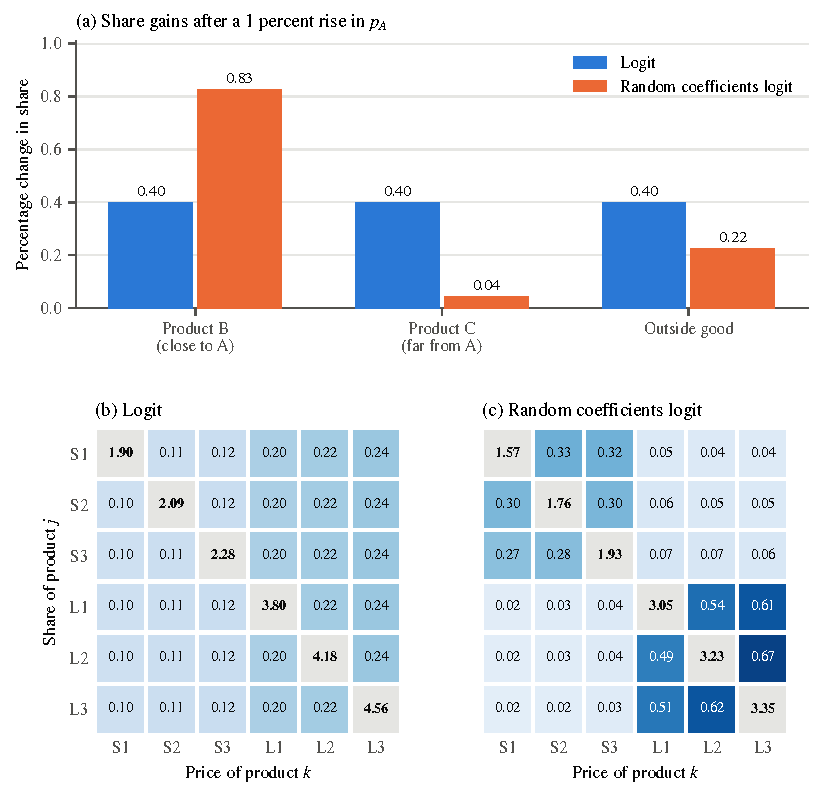
\includegraphics[width=\textwidth]{figures/ch08/fig_substitution.pdf}
\caption{Substitution in the logit and random coefficients logit models. Panel (a): three products with
characteristic $x = (1.0, 0.9, -1.0)$, prices $p = (1, 1, 1)$ and shares $s = (0.20, 0.10, 0.10)$, so A and B are
close and B and C have equal shares. Bars show the percentage change in the shares of B, C and the outside good
after a 1 percent rise in $p_A$. The random coefficients model has normal random coefficients on the constant
(standard deviation 1.0) and on $x$ (standard deviation 2.5), and $\alpha = 2$ in both models. Panels (b) and
(c): six products with shares 0.05, sizes $(-1.0, -0.9, -0.8, 0.8, 0.9, 1.0)$ and prices $(1.0, 1.1, 1.2, 2.0, 2.2,
2.4)$. Cell $(j, k)$ is the elasticity of the share of $j$ with respect to the price of $k$. Grey diagonal cells
report the positive own elasticity $\varepsilon_j = -\varepsilon_{jj}$. The random coefficients model has standard
deviations 1.0 (constant), 2.0 (size) and 0.5 (price), with $\alpha_i = 2 - 0.5\nu_{ip}$. Both models fit the same
shares. Computed by \texttt{figures/ch08/src/fig\_substitution.py}.}
\label{fig:08-substitution}
\end{figure}

\subsection{Further contrasts}\label{sec:08-contrasts}

The vertical model of \cref{ch:discrete} also has heterogeneous consumers, but only along one dimension. Cross
elasticities are then nonzero only between products adjacent in the price ranking.
\citet[p.~852]{BerryLevinsohnPakes1995} give an example. Suppose the ranking contains a \$24,998 family station
wagon, a \$24,999 sports car and a \$25,000 family station wagon, in that order. The vertical model guarantees
that the two wagons are not substitutes for each other, while the sports car is a substitute for both. Random
coefficients on several characteristics let products be differentiated in several dimensions at once.

\begin{remark}[Fitting a logit when tastes are heterogeneous]\label{rem:08-logit-misspec}
Suppose the data come from the random coefficients model and we estimate the logit regression $\ln s_{jt} -
\ln s_{0t} = x_{jt}\beta - \alpha p_{jt} + \text{error}$ by instrumental variables. Write $r_{jt} = \ln s_{jt} -
\ln s_{0t} - \delta_{jt}$ for the gap between the logit inversion and the true mean utility. The regression error is
$\xi_{jt} + r_{jt}$. The gap depends on prices, because less price-sensitive consumers sort into expensive
products. By \eqref{eq:08-elasticity-buyers}, the log share of an expensive product falls with its price at a rate
set by the low price sensitivity of its buyers, more slowly than $\alpha$. An instrument that moves prices, such
as a cost shifter, also moves $r_{jt}$. The instrument is then correlated with the regression error even if it is
independent of $\xi_{jt}$. When less price-sensitive consumers sort into expensive products in this way, the
logit price coefficient tends to be biased toward zero. The argument is heuristic, and \cref{sec:08-worked}
measures the correlation and the bias in a simulated market.
\end{remark}

\begin{remark}[Price changes and product deletions]\label{rem:08-deletion}
\citet[p.~94]{BerryLevinsohnPakes2004} distinguish two substitution patterns. After a price rise, only a selected
group of a product's buyers leave, the more price-sensitive ones. After the product is deleted, all of its buyers
must choose again. The model makes the difference explicit. If $j$ is removed, a consumer who would have bought $j$
chooses $k$ with probability $\frac{s_{ik}}{1 - s_{ij}}$ by \cref{rem:08-iia}. The fraction of $j$'s buyers who move
to $k$ is therefore
\begin{equation}\label{eq:08-deletion-diversion}
  D^{\text{del}}_{jk} = \int \frac{s_{ij}}{s_j}\, \frac{s_{ik}}{1 - s_{ij}}\, \dd F.
\end{equation}
It averages the same individual diversion ratios as \eqref{eq:08-diversion-average}, with weights
$\frac{s_{ij}}{s_j}$ instead of $\varpi_{ij}$. The two coincide in the logit, where both equal $\frac{s_k}{1 -
s_j}$. With heterogeneous tastes they differ, and the deletion pattern is the relevant one for questions such as the
closing of a brand (\cref{sec:08-blp04}).
\end{remark}

\section{Computing the share integral by simulation}\label{sec:08-simulation}

The share integral \eqref{eq:08-share-integral} has the dimension of $(D_i, \nu_i)$, the number of demographics
plus the number of random coefficients. It has no closed form once that dimension exceeds zero, and
\citet[p.~866]{BerryLevinsohnPakes1995} note that numerical integration becomes difficult once the dimension grows
beyond two or three. They replace the integral by a simulation estimator, a technique that
\citet{Pakes1986} introduced as aggregation by simulation \citep[p.~848]{BerryLevinsohnPakes1995}. This section
describes the standard simulator, its error, the importance sampler of \citet{BerryLevinsohnPakes1995}, the
treatment of demographics, deterministic alternatives, and safe numerical evaluation.

\subsection{The smooth simulator}\label{sec:08-smooth-simulator}

Draw $n_s$ consumers $(D_i, \nu_i)$, $i = 1, \dots, n_s$, from $F_{Dt} \times F_\nu$. The \emph{smooth
simulator} of the share of product $j$ is the average of the individual logit probabilities
\citep[eq.~(6.10)]{BerryLevinsohnPakes1995}:
\begin{equation}\label{eq:08-smooth-simulator}
  s^{n_s}_{jt}(\delta_t; \theta_2) = \frac{1}{n_s}\sum_{i=1}^{n_s} s_{ijt}.
\end{equation}
With diagonal $\Sigma$, each term is written out as
\begin{equation*}
  s_{ijt} = \frac{\exp\bigl(\delta_{jt} + \sum_{k} \tilde x_{jtk}(\sigma_k\nu_{ik} + \pi_{k1}D_{i1} + \cdots
            + \pi_{kd}D_{id})\bigr)}
         {1 + \sum_{m \in \mathcal{J}_t}\exp\bigl(\delta_{mt} + \sum_{k} \tilde x_{mtk}(\sigma_k\nu_{ik}
          + \pi_{k1}D_{i1} + \cdots + \pi_{kd}D_{id})\bigr)},
\end{equation*}
which gives equation (11) of \citet{Nevo2000a}. The sums over $k$ run over the characteristics that carry random
coefficients.

The simulator has four properties \citep[p.~865]{BerryLevinsohnPakes1995}. It is unbiased for $s_{jt}$. Its
values are positive. Together with the simulated outside share $\frac{1}{n_s}\sum_i s_{i0t}$ the shares sum to
one. It is a smooth function of $(\delta_t, \theta_2)$. Because the extreme value shocks are integrated
analytically, its variance comes only from the draws of $(D_i, \nu_i)$. The next lemma makes the last point precise
by comparing it with the \emph{frequency simulator}, which also draws the shocks $\epsilon_{ijt}$ and counts the
simulated consumers who choose $j$.

\begin{lemma}[Smooth versus frequency simulator]\label{lem:08-smooth}
Let $s^{\text{freq}}_j = \frac{1}{n_s}\sum_{i=1}^{n_s}\indic\{j = \argmax_{k} u_{ik}\}$, where each simulated
consumer has draws $(D_i, \nu_i, \epsilon_{i0}, \dots, \epsilon_{iJ})$. Both simulators are unbiased for $s_j$, and
\begin{equation}\label{eq:08-rao-blackwell}
  \Var\bigl(s^{\text{freq}}_j\bigr) = \frac{s_j(1 - s_j)}{n_s}
  = \Var\bigl(s^{n_s}_j\bigr) + \frac{1}{n_s}\E\bigl[s_{ij}(1 - s_{ij})\bigr],
  \qquad \Var\bigl(s^{n_s}_j\bigr) = \frac{\Var(s_{ij})}{n_s}.
\end{equation}
\end{lemma}

\begin{proof}
Let $I_{ij}$ be the indicator that simulated consumer $i$ chooses $j$. Conditional on $(D_i, \nu_i)$, it is a
Bernoulli variable with mean $s_{ij}$. By the law of iterated expectations, $\E[I_{ij}] = \E[s_{ij}] = s_j$, so
both simulators are unbiased. Unconditionally $I_{ij}$ is Bernoulli with mean $s_j$, so $\Var(I_{ij}) = s_j(1 -
s_j)$. The law of total variance gives
\begin{equation*}
  \Var(I_{ij}) = \E\bigl[\Var(I_{ij} \mid D_i, \nu_i)\bigr] + \Var\bigl(\E[I_{ij} \mid D_i, \nu_i]\bigr)
              = \E\bigl[s_{ij}(1 - s_{ij})\bigr] + \Var(s_{ij}).
\end{equation*}
The draws are independent across simulated consumers, so dividing by $n_s$ gives the variances of the two
averages.
\end{proof}

The smooth simulator is the conditional expectation of the frequency simulator given the draws of $(D_i,
\nu_i)$. Conditioning removes the variance $\frac{1}{n_s}\E[s_{ij}(1 - s_{ij})]$. The frequency simulator has two
further defects. It is a step function of $(\delta, \theta_2)$, with zero derivatives almost everywhere and jumps
in between, so gradient-based optimizers cannot use it. It also equals zero with positive probability for small
products, and then $\ln s^{\text{freq}}_j$ is undefined and the share equations cannot be inverted.

\subsection{Simulation error in log shares}\label{sec:08-simbias}

The estimator of \cref{sec:08-gmm} uses the simulated shares through their logarithms, in the inversion step. An
unbiased simulator of $s_j$ is a biased simulator of $\ln s_j$. Let $c_j = \frac{\sqrt{\Var(s_{ij})}}{s_j}$ be the
coefficient of variation of the individual purchase probabilities of product $j$.

\begin{proposition}[Bias of the simulated log share]\label{prop:08-simbias}
Let $s^{n_s}_j$ be the smooth simulator with independent draws, and suppose $\Var(s_{ij}) > 0$.
\begin{enumerate}[label=(\roman*)]
  \item $\E[s^{n_s}_j] = s_j$ and $\Var(s^{n_s}_j) = \frac{\Var(s_{ij})}{n_s}$.
  \item $\E[\ln s^{n_s}_j] < \ln s_j$.
  \item If $s_{ij} \ge \underline{s} > 0$ for all $(D_i, \nu_i)$, then
    \begin{equation}\label{eq:08-simbias}
      \E\bigl[\ln s^{n_s}_j\bigr] - \ln s_j = -\frac{\Var(s^{n_s}_j)}{2s_j^2} + O\bigl(n_s^{-\frac{3}{2}}\bigr)
      = -\frac{c_j^2}{2n_s} + O\bigl(n_s^{-\frac{3}{2}}\bigr).
    \end{equation}
\end{enumerate}
\end{proposition}

\begin{proof}
Part (i) restates \cref{lem:08-smooth}. For (ii), the logarithm is strictly concave and $s^{n_s}_j$ is not
degenerate because $\Var(s_{ij}) > 0$. Jensen's inequality gives $\E[\ln s^{n_s}_j] < \ln\E[s^{n_s}_j] = \ln s_j$.

For (iii), write $Y = s^{n_s}_j$ and expand $\ln Y$ around $s_j$ with the Lagrange form of the remainder:
\begin{equation*}
  \ln Y = \ln s_j + \frac{Y - s_j}{s_j} - \frac{(Y - s_j)^2}{2s_j^2} + \frac{(Y - s_j)^3}{3\bar Y^3},
\end{equation*}
where $\bar Y$ lies between $Y$ and $s_j$. Take expectations. The linear term has mean zero by (i). The quadratic
term has mean $-\frac{\Var(Y)}{2s_j^2}$. Both $Y$ and $s_j$ are at least $\underline{s}$, so $\bar Y \ge
\underline{s}$ and the remainder is bounded in absolute value by $\frac{\E|Y - s_j|^3}{3\underline{s}^3}$. For an
average of $n_s$ independent bounded variables, $\E|Y - s_j|^3 \le (\E(Y - s_j)^4)^{\frac{3}{4}}$, and the fourth
central moment of such an average is $O(n_s^{-2})$. The remainder is therefore $O(n_s^{-\frac{3}{2}})$.
Substituting $\Var(Y) = \frac{\Var(s_{ij})}{n_s}$ gives the second form.
\end{proof}

The lower bound in (iii) holds when the support of $(D_i, \nu_i)$ is bounded. With normal tastes it fails, but the
second-order term still describes the bias well in practice, as the evidence below shows. The bias is of order
$\frac{1}{n_s}$ and its size is governed by $c_j$. The coefficient of variation is large when the purchase
probability of $j$ is concentrated on a small group of consumers. Small niche products have the largest $c_j$ and
the largest bias.

The bias passes to the mean utilities. For given $\theta_2$, the inversion of \cref{sec:08-inversion} finds the
$\hat\delta_t$ that solves $s^{n_s}_t(\hat\delta_t; \theta_2) = s^{\text{obs}}_t$. A first-order expansion around
the true $\delta_t$, using the nonsingular Jacobian of \cref{prop:08-shares}, gives
\begin{equation}\label{eq:08-delta-error}
  \hat\delta_t - \delta_t \approx -\Bigl[\frac{\partial s_t}{\partial \delta_t^\T}\Bigr]^{-1}
  \bigl(s^{n_s}_t(\delta_t; \theta_2) - s_t(\delta_t; \theta_2)\bigr).
\end{equation}
The leading term has mean zero and variance of order $\frac{1}{n_s}$. This is the simulation component of the
asymptotic variance of the estimator in \cref{sec:08-gmm}, which \citet[p.~859]{BerryLevinsohnPakes1995} call
$V_3$. The second-order terms, like those in \eqref{eq:08-simbias}, add a bias of order $\frac{1}{n_s}$. At the
true $\delta_t$ the simulated log shares are too low on average, so the inversion tends to push $\hat\delta_t$
up, most for products with dispersed purchase probabilities.

The bias has a consequence for estimation that the variance does not have. Independent draws across markets make
the leading simulation errors independent across markets. They average out of the sample moments as the number of
markets grows. The bias of order $\frac{1}{n_s}$ is present in every market with the same sign, and it does not
average out. Consistency therefore requires $n_s$ to grow with the sample. \citet[p.~859]{BerryLevinsohnPakes1995} cite asymptotic
results of Berry and Pakes, then in progress, for their utility specification. These results require the number
of consumers and the number of simulation draws to grow at the rate $J^3$.
\citet{BerryLintonPakes2004} develop limit theorems of this kind for asymptotics in the number of products.
\citet[Section~4.4]{BerryPakes2007} report the rates that these theorems require. The number of draws must grow at
the slower rate $J^2$ in logit-style models and at rate $J$ in the vertical model (\cref{sec:08-pcm}). BLP's
rate refers to their own utility specification and to results that were still in progress.

\Cref{fig:08-simerror} and \cref{tab:08-simdelta} quantify these effects in one simulated market with five inside
products, shares $(0.10, 0.05, 0.03, 0.015, 0.005)$ and an outside share of 0.80. The market has normal random
coefficients on a constant, a characteristic and price. The coefficients of variation $c_j$ are 1.49, 0.97, 0.94,
1.51 and 2.99. The product with share 0.10 is expensive and bought mostly by consumers who like its
characteristics, so its $c_j$ exceeds those of the two middle products.

\begin{figure}[htbp]
\centering
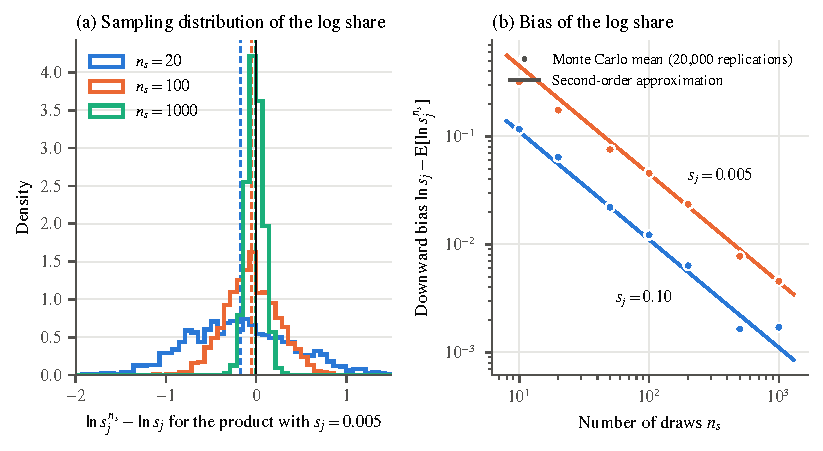
\includegraphics[width=\textwidth]{figures/ch08/fig_simulation.pdf}
\caption{Simulation error in simulated log shares, for one market with outside share 0.80 and inside shares
$(0.10, 0.05, 0.03, 0.015, 0.005)$. Tastes are normal with standard deviations 1.0 on the constant, 1.5 on a characteristic $x =
(1.0, 0.5, 0.0, -0.5, -1.0)$ and 0.5 on price, prices are $(2.0, 1.6, 1.2, 1.0, 0.8)$ and $\alpha = 2$. True shares
come from a 64,000-node Gauss-Hermite rule and agree with $10^6$ pseudo-random draws to within 0.002 in relative
terms. Panel (a): distribution of $\ln s^{n_s}_j - \ln s_j$ for the product with share 0.005 over 2,000 replications
with fresh pseudo-random draws. Dashed lines mark the means. Panel (b): downward bias of the simulated log share
(dots, 20,000 replications per $n_s$) and the second-order approximation $\frac{\Var(s_{ij})}{2n_s s_j^2}$ of
\cref{prop:08-simbias} (lines). Computed by \texttt{figures/ch08/src/fig\_simulation.py}.}
\label{fig:08-simerror}
\end{figure}

Panel (a) of \cref{fig:08-simerror} shows the sampling distribution of the simulated log share of the smallest
product. With 20 draws it is wide and skewed to the left, and its mean lies well below zero. With 1,000 draws it is
concentrated near zero. Panel (b) shows that the downward bias falls like $\frac{1}{n_s}$. The second-order
approximation is accurate from about 50 draws for the product with share 0.10 and from about 100 draws for the
product with share 0.005. For the product with share 0.005, the bias is 0.175
with 20 draws (approximation 0.224), 0.046 with 100 draws (approximation 0.045), and 0.005 with 1,000 draws
(approximation 0.004). With 10 or 20 draws the approximation overstates the bias of the smallest product, because
higher-order terms matter when the simulator is very noisy.

\begin{table}[htbp]
\centering
\caption{Error in the inverted mean utility caused by simulation}\label{tab:08-simdelta}
\begin{tabular}{lccccc}
\toprule
 & \multicolumn{5}{c}{Market share of the product} \\
\cmidrule(lr){2-6}
Draws $n_s$ & 0.10 & 0.05 & 0.03 & 0.015 & 0.005 \\
\midrule
20    & 0.037 & 0.010 & 0.021 & 0.063 & 0.198 \\
      & (0.547) & (0.362) & (0.273) & (0.368) & (0.627) \\
100   & $-0.008$ & $-0.009$ & $-0.008$ & $-0.006$ & 0.015 \\
      & (0.250) & (0.163) & (0.126) & (0.177) & (0.328) \\
1,000 & 0.003 & 0.001 & $-0.000$ & $-0.002$ & $-0.006$ \\
      & (0.077) & (0.051) & (0.040) & (0.056) & (0.104) \\
\bottomrule
\end{tabular}

\smallskip
\begin{minipage}{0.86\linewidth}
\footnotesize Notes: Each entry is the mean of $\hat\delta_j - \delta_j$ over 500 replications, with its standard
deviation in parentheses. In each replication we draw $n_s$ consumers and solve $s^{n_s}(\hat\delta; \theta_2) =
s$ by the contraction of \cref{sec:08-inversion}, at the true $\theta_2$ and the true shares. The market is the one
of \cref{fig:08-simerror}. The standard error of each mean is its standard deviation divided by
$\sqrt{500} \approx 22.4$. Computed by \texttt{figures/ch08/src/fig\_simulation.py}.
\end{minipage}
\end{table}

\Cref{tab:08-simdelta} turns to the mean utilities. With 20 draws, the inverted $\hat\delta_j$ of the product
with share 0.005 is too high by 0.198 on average, with a standard error of $\frac{0.627}{22.4} = 0.028$. The
product with share 0.015 is too high by 0.063 (standard error 0.016). These are the upward biases predicted
above. Their size is small relative to the standard deviations, which range from 0.27 to 0.63. The standard
deviations fall roughly like $\frac{1}{\sqrt{n_s}}$, from about 0.4 on average with 20 draws to about 0.07 with
1,000 draws. With 100 or more draws the mean errors are within two standard errors of zero.

\subsection{Draws in practice}\label{sec:08-draws}

Three rules govern the use of simulation draws in estimation.

The draws are taken once, before estimation, and held fixed while the optimizer varies the parameters. If new
draws were taken at each evaluation, the objective would be a different random function each time it is
evaluated. The search would chase the simulation noise and fail to converge. The asymptotic theory of simulation
estimators also requires draws that do not change with $\theta$ \citep[p.~867]{BerryLevinsohnPakes1995},
\citep{PakesPollard1989}.

Draws are usually independent across markets. Then simulation errors are independent across markets and their
leading terms average out of the moments, so a moderate number of draws per market can suffice when markets are
many. The bias term of \cref{prop:08-simbias} is the exception, as explained above. \citet{BerryLevinsohnPakes1995}
instead hold the same draws of $(\nu_{iy}, \nu_{i0}, \dots, \nu_{iK})$ fixed over all years of their panel, while the
income distribution shifts through $m_t$ \citep[p.~868]{BerryLevinsohnPakes1995}.

The number of draws trades accuracy against computing time. \citet[pp.~538, 540]{Nevo2000a} draws 20 consumers per market
in his illustrative application and notes that more draws or better simulation methods would improve efficiency.
The evidence above shows that 20 pseudo-random draws leave sizable errors in the shares of small products.

Demographics need their own draws. \citet[p.~868, n.~21]{BerryLevinsohnPakes1995} tried taking draws of income from the
CPS for each year. They found that this less restrictive procedure gave imprecise simulators, in particular for
changes in the upper tail of the income distribution. They therefore kept a lognormal income distribution with
year-specific means. They did not estimate a separate standard deviation for each year because those estimates were
imprecise. \citet[n.~25]{Nevo2001} samples 40 individuals from the CPS for each city and year, 200 for each city in
total. He reports that the results were robust to increasing the number of individuals where possible. Empirical
draws of $D_i$ are combined with independent draws of $\nu_i$ from $F_\nu$.

\subsection{Importance sampling}\label{sec:08-importance}

Pseudo-random draws from $F_\nu$ waste effort when few consumers buy any inside product. In the car market most
households do not buy a new car in a given year. Most draws then have purchase probabilities near zero and
contribute little to any share. \citet[Section~6.3]{BerryLevinsohnPakes1995} reduce the variance of the simulator by
importance sampling. To keep notation light, let $\nu$ collect all simulated consumer characteristics, with density
$p_0(\nu)$, and write $f_j(\nu, \theta)$ for the individual choice probability \eqref{eq:08-individual-share}.

Take any density $h(\nu, \theta)$ that is positive wherever $p_0$ is. The share can be rewritten as
\citep[eq.~(6.11)]{BerryLevinsohnPakes1995}
\begin{equation}\label{eq:08-importance-identity}
  s_j(\theta) = \int f_j(\nu, \theta)\, p_0(\nu)\, \dd\nu
  = \int \Bigl[\frac{f_j(\nu, \theta)\, p_0(\nu)}{h(\nu, \theta)}\Bigr] h(\nu, \theta)\, \dd\nu.
\end{equation}
Averaging the bracketed term over draws from $h$ gives an unbiased simulator. Its variance is the variance of the
bracketed term under $h$, divided by the number of draws. The variance is zero for the choice
\citep[eq.~(6.12)]{BerryLevinsohnPakes1995}
\begin{equation}\label{eq:08-optimal-importance}
  h^*_j(\nu, \theta) = \frac{f_j(\nu, \theta)\, p_0(\nu)}{s_j(\theta)},
\end{equation}
because the bracketed term then equals $s_j(\theta)$ for every draw. This density over-samples consumers whose
characteristics make them likely to buy product $j$.

The optimal density cannot be used directly, for three reasons \citep[pp.~866--867]{BerryLevinsohnPakes1995}. It
requires $s_j(\theta)$, the integral we want to compute. It depends on $\theta$, while the draws must stay fixed as
the optimizer varies $\theta$. It differs across products, so each simulated share would come from its own draws.
The inversion of \cref{sec:08-inversion} instead computes all shares from one distribution of consumers.

\citeauthor{BerryLevinsohnPakes1995} build a feasible version from a preliminary estimate $\theta'$, obtained with the
smooth simulator. They target the probability of buying some car, $\bar f(\nu, \theta') = \sum_{j=1}^{J} f_j(\nu,
\theta')$, whose integral is the total inside share $\bar s(\theta') = 1 - s_0(\theta')$. Draws come from $p_0$ by
acceptance and rejection: a draw $\nu$ is accepted with probability $\bar f(\nu, \theta')$. By Bayes' rule the
density of an accepted draw is
\begin{equation}\label{eq:08-accepted-density}
  h(\nu) = \frac{p_0(\nu)\, \Pr(\text{accept} \mid \nu)}{\Pr(\text{accept})}
         = \frac{p_0(\nu)\, \bar f(\nu, \theta')}{\int p_0(\nu')\, \bar f(\nu', \theta')\, \dd\nu'}
         = \frac{p_0(\nu)\, \bar f(\nu, \theta')}{\bar s(\theta')}.
\end{equation}
Substituting this $h$ into \eqref{eq:08-importance-identity} gives the bracketed term $\frac{\bar
s(\theta')}{\bar f(\nu, \theta')}f_j(\nu, \theta)$. With $n_s$ accepted draws $\nu_1, \dots, \nu_{n_s}$, the
simulator is \citep[eq.~(6.13)]{BerryLevinsohnPakes1995}\footnote{Equation (6.13) of
\citet{BerryLevinsohnPakes1995} is printed without the factor $\frac{1}{n_s}$. The average is needed for the
simulator to be unbiased.}
\begin{equation}\label{eq:08-blp-importance}
  s_j\bigl[\theta, P^*_h(\theta')_{n_s}\bigr] = \frac{1}{n_s}\sum_{i=1}^{n_s}
  \frac{\bar s(\theta')}{\bar f(\nu_i, \theta')}\, f_j(\nu_i, \theta).
\end{equation}
The draws are fixed once $\theta'$ is chosen, and every share uses the same draws. Since $\bar s(\theta')$ is computed
only once, it can be computed with many draws at little cost.

The construction removes one source of noise. At $\theta = \theta'$ the weighted integrand is $\bar s(\theta')$ times
$\frac{f_j(\nu, \theta')}{\bar f(\nu, \theta')}$, the probability of choosing $j$ given that the consumer buys some
car. That ratio lies between zero and one. Summed over $j$ it equals $\bar s(\theta')$ for every draw, so the
simulated total inside share has no simulation error at all. The variation that remains comes only from which car
a buyer chooses.

Common draws do not make the simulated shares add up to one, although \citet[p.~867]{BerryLevinsohnPakes1995} use
them for that purpose. Write $w_i = \frac{\bar s(\theta')}{\bar f(\nu_i, \theta')}$ for the weight of draw $i$ and
$\bar w = \frac{1}{n_s}\sum_{i} w_i$ for the mean weight. Applying \eqref{eq:08-blp-importance} to all $J + 1$
options and using $\sum_{j=0}^{J} f_j = 1$ gives $\sum_{j=0}^{J} s_j = \bar w$. Each weight has expectation one under
$h$, so $\bar w$ equals one only on average. The contraction uses only the inside shares, and this random total does
not break it. The simulated inside shares equal $\bar w$ times the shares computed under the probability weights
$\frac{w_i}{n_s\bar w}$. \Cref{thm:08-berry94}, applied to this distribution of draws, gives a unique solution
whenever the observed inside shares sum to less than $\bar w$. With a small inside share and many draws, $\bar w$ is
close to one and the condition is mild. Self-normalizing the weights would make the shares sum to one exactly, at
the cost of a finite-sample bias that vanishes as $n_s$ grows.

\Cref{tab:08-importance} compares the two simulators in the market of \cref{fig:08-simerror}, whose total inside share
is 0.20. With 100 draws, importance sampling cuts the relative root mean squared error of the largest product's share
from 15.3 to 4.8 percent. For the second product it falls from 10.0 to 2.8 percent. The gains are small for
the two smallest products, from 15.0 to 13.5 percent and from 29.4 to 25.5 percent. Their buyers are a small subset of
car buyers, so conditioning on buying some car leaves most of their simulation noise in place. A preliminary
estimate that understates every standard deviation by 20 percent loses little of the gain.

\begin{table}[htbp]
\centering
\caption{Smooth simulator and importance sampling: relative root mean squared error (percent)}\label{tab:08-importance}
\begin{tabular}{lccccc}
\toprule
 & \multicolumn{5}{c}{Market share of the product} \\
\cmidrule(lr){2-6}
Simulator & 0.10 & 0.05 & 0.03 & 0.015 & 0.005 \\
\midrule
Smooth simulator & 15.31 & 9.95 & 9.52 & 14.98 & 29.35 \\
Importance sampling, $\theta' = \theta$ & 4.83 & 2.84 & 6.79 & 13.51 & 25.46 \\
Importance sampling, $\sigma' = 0.8\sigma$ & 5.55 & 2.90 & 6.35 & 13.28 & 26.31 \\
\bottomrule
\end{tabular}

\smallskip
\begin{minipage}{0.9\linewidth}
\footnotesize Notes: Each entry is $100\sqrt{\E\bigl[(\frac{\hat s_j}{s_j} - 1)^2\bigr]}$ over 1,000 replications
with $n_s = 100$ draws (accepted draws for importance sampling). The importance sampler is
\eqref{eq:08-blp-importance}. In the last row the preliminary estimate $\theta'$ multiplies every standard deviation by
0.8 and uses the mean utilities that fit the shares at those values. The acceptance rate equals the total inside share,
0.20. Mean errors of the importance sampler are below 0.6 percent in absolute value. Computed by
\texttt{figures/ch08/src/fig\_simulation.py}.
\end{minipage}
\end{table}

\subsection{Quadrature and quasi-Monte Carlo}\label{sec:08-quadrature}

Pseudo-random draws are not the only way to approximate \eqref{eq:08-share-integral}. Any rule of the form $\sum_q w_q
s_{ij}(\nu_q)$ with nodes $\nu_q$ and weights $w_q$ can replace the simple average, and the share equations and
their inversion are unchanged.

A \emph{Gauss-Hermite product rule} uses, in each dimension, the $Q$ nodes and weights that integrate polynomials of
degree up to $2Q - 1$ exactly against the normal density. For a standard normal variable,
\begin{equation}\label{eq:08-gauss-hermite}
  \int g(\nu)\, \phi(\nu)\, \dd\nu \approx \sum_{q=1}^{Q} \frac{w_q}{\sqrt{\pi}}\, g\bigl(\sqrt{2}\, x_q\bigr),
\end{equation}
where $(x_q, w_q)$ are the Gauss-Hermite nodes and weights for the weight function $e^{-x^2}$. The product rule takes
all combinations of the one-dimensional nodes, so it needs $Q^{L}$ nodes for $L$ random coefficients. It is very
accurate for smooth integrands in low dimensions and becomes expensive quickly as $L$ grows. \emph{Sparse grids}
combine lower-order product rules so that the number of nodes grows polynomially in $L$ \citep{HeissWinschel2008}.
\emph{Quasi-Monte Carlo} methods, such as Halton sequences, replace pseudo-random draws by deterministic sequences that
fill the unit cube more evenly. The points are mapped to normal draws by the inverse distribution function
\citep[Section~9.3.3]{Train2009}.
A randomly scrambled Halton sequence keeps the even coverage and allows replications. The
\texttt{pyblp} software of \citet[Section~3]{ConlonGortmaker2020} implements all of these rules. By default it
scrambles each Halton sequence and discards its first 1,000 points.

\Cref{tab:08-integration} compares the three approaches in the market of \cref{fig:08-simerror}, which has three random
coefficients. At equal numbers of nodes, scrambled Halton draws reduce the error of pseudo-random draws by a factor of
about 2 to 20, and the gain grows with the number of nodes. The Gauss-Hermite product rule is accurate to a few hundredths of a percent with 125 nodes and to about
$10^{-5}$ percent with 1,000 nodes. The product rule's advantage shrinks with more random coefficients. It also shrinks when
demographic distributions are known only through empirical draws, which quadrature cannot use directly.

\begin{table}[htbp]
\centering
\caption{Accuracy of integration rules: relative error of simulated shares (percent)}\label{tab:08-integration}
\begin{tabular}{lccc}
\toprule
 & \multicolumn{3}{c}{Number of nodes} \\
\cmidrule(lr){2-4}
Rule & 125 & 1,000 & 8,000 \\
\midrule
\multicolumn{4}{l}{\textit{Product with $s_j = 0.10$}} \\
Pseudo-random draws & 12.45 & 4.84 & 1.56 \\
Scrambled Halton draws & 3.41 & 0.53 & 0.076 \\
Gauss-Hermite product rule & $2.9 \times 10^{-2}$ & $1.9 \times 10^{-5}$ & $3.0 \times 10^{-10}$ \\
\addlinespace
\multicolumn{4}{l}{\textit{Product with $s_j = 0.005$}} \\
Pseudo-random draws & 27.63 & 10.29 & 3.30 \\
Scrambled Halton draws & 13.38 & 2.45 & 0.46 \\
Gauss-Hermite product rule & $4.5 \times 10^{-2}$ & $2.5 \times 10^{-5}$ & $6.2 \times 10^{-10}$ \\
\bottomrule
\end{tabular}

\smallskip
\begin{minipage}{0.8\linewidth}
\footnotesize Notes: Market of \cref{fig:08-simerror}, with three normal random coefficients. Entries for random rules
are relative root mean squared errors over 200 replications. Entries for the Gauss-Hermite rule, which uses 5, 10 and
20 nodes per dimension, are absolute relative errors against a rule with 40 nodes per dimension. Computed by
\texttt{figures/ch08/src/fig\_simulation.py}.
\end{minipage}
\end{table}

\subsection{Safe numerical evaluation}\label{sec:08-overflow}

Evaluating \eqref{eq:08-individual-share} naively can overflow. Mean utilities and random coefficient terms can be
large during the search, and $e^{V}$ exceeds the largest double-precision number once $V$ exceeds about 709. The
logit formula is invariant to subtracting the same constant from every utility of a consumer, including the zero
utility of the outside good. Let $m_i = \max\{0, \max_k V_{ik}\}$. Then
\begin{equation}\label{eq:08-logsumexp}
  s_{ij} = \frac{e^{V_{ij} - m_i}}{e^{-m_i} + \sum_k e^{V_{ik} - m_i}}, \qquad
  \ln s_{ij} = V_{ij} - m_i - \ln\Bigl(e^{-m_i} + \sum_k e^{V_{ik} - m_i}\Bigr).
\end{equation}
Every exponent is now at most zero, and at least one term in the denominator equals one, so neither overflow nor
division by zero can occur. The second expression, the log-sum-exp form, also gives accurate log shares for very
small probabilities. All computations in this chapter use \eqref{eq:08-logsumexp}.
